% !TEX program = xelatex
\documentclass[UTF8, 12pt, a4paper]{ctexart}

% ── 宏包 ──────────────────────────────────────────────────────────────────
\usepackage[left=2.5cm, right=2.5cm, top=2.8cm, bottom=2.5cm]{geometry}
\usepackage{graphicx}
\usepackage{booktabs}
\usepackage{amsmath, amssymb}
\usepackage{float}
\usepackage{caption}
\usepackage{subcaption}
\usepackage{enumitem}
\usepackage{tabularx}
\usepackage{multirow}
\usepackage{color, xcolor}
\usepackage{setspace}
\usepackage{cite}
\usepackage{hyperref}

\hypersetup{
    colorlinks=true,
    linkcolor=blue!60!black,
    citecolor=blue!60!black,
    urlcolor=blue!60!black,
    pdfencoding=auto,
}

\graphicspath{{figures/}{html_figures/}}
\onehalfspacing

% ── 标题信息 ──────────────────────────────────────────────────────────────
\title{\textbf{基于 Coursera MOOC 平台的\\在线学习行为数据分析与成绩预测研究}}
\author{李\ 涛 \\[0.4em]
\normalsize 清华大学\ 工程物理系 \\
\normalsize 北京大学《教育与人工智能》课程（2026 年春）\\
\normalsize 指导教师：贾积有\ 教授}
\date{2026 年 4 月}

% ════════════════════════════════════════════════════════════════════════════
\begin{document}
\maketitle
\thispagestyle{empty}

% ── 摘要 ──────────────────────────────────────────────────────────────────
\begin{abstract}
随着大规模在线开放课程（MOOC）的快速发展，如何利用学习行为数据优化教学效果成为教育数据挖掘领域的重要课题。
本文基于Coursera平台某课程的15,168条学生会话数据，从描述性统计、相关性分析、聚类分析、回归预测和分类预测五个维度，系统研究了学生在线学习行为与最终成绩之间的关系。
研究发现：（1）在线时长、活跃天数和页面浏览次数与成绩呈显著正相关（$r>0.67$）；
（2）K-Means聚类将学生分为三类群体，高活跃群体平均成绩显著高于低活跃群体；
（3）线性回归模型取得$R^2=0.614$的预测效果；
（4）MLP神经网络在二分类任务中准确率达到84.57\%。
此外，本文还配套实现了一个交互式可视化与AI问答平台\textbf{EduAnalytics}，支持用户拖拽上传CSV数据、一键完成全流程分析、并基于当前数据与大语言模型进行自然语言问答。
研究结果及所开发的平台为在线教育平台的学习预警和个性化干预提供了数据支撑和工具支持。

\vspace{1em}
\noindent\textbf{关键词：} MOOC；学习行为分析；教育数据挖掘；成绩预测；聚类分析；可视化平台
\end{abstract}

\newpage
\setcounter{page}{1}
\tableofcontents
\newpage

% ══════════════════════════════════════════════════════════════════════════
\section{引言}
% ══════════════════════════════════════════════════════════════════════════

近年来，大规模在线开放课程（Massive Open Online Course, MOOC）已成为全球高等教育的重要组成部分\cite{jordan2015mooc}。Coursera、edX、学堂在线等平台汇聚了数千万学习者，为教育公平化和终身学习提供了前所未有的机遇。然而，MOOC面临的一个核心挑战是高退课率和低完成率——相关研究表明，MOOC的平均完成率仅为5\%--15\%\cite{khalil2014mooc}。

教育数据挖掘（Educational Data Mining, EDM）和学习分析（Learning Analytics, LA）为解决这一问题提供了技术路径\cite{romero2020edm}。通过分析学生在平台上的行为数据——如视频观看、页面浏览、论坛参与等——可以发现影响学业表现的关键因素，进而实现学习预警和个性化干预。

本研究基于Coursera平台某课程的真实学生行为数据，围绕以下研究问题展开：
\begin{enumerate}[label=RQ\arabic*.]
    \item 哪些在线学习行为特征与最终成绩显著相关？
    \item 基于行为特征能否对学生进行有效的群体划分？
    \item 能否利用行为特征对学生成绩进行定量预测和高低分分类？
\end{enumerate}

本文的主要贡献包括：（1）对MOOC学习行为数据进行了系统的多角度分析；（2）对比了多种机器学习模型在成绩预测任务上的表现；（3）结合分析结果提出了面向教学实践的建议；（4）设计并实现了配套的交互式数据分析与AI问答平台\textbf{EduAnalytics}，将离线脚本分析工作流升级为可交互、可复用的Web工具。

% ══════════════════════════════════════════════════════════════════════════
\section{数据与方法}
% ══════════════════════════════════════════════════════════════════════════

\subsection{数据来源}

本研究使用的数据集来自Coursera平台的某MOOC课程，包含15,168条学生会话记录。每条记录对应一名学生在该课程中的完整学习行为数据和最终成绩。

\subsection{数据字段说明}

数据集包含的主要字段如表\ref{tab:fields}所示。

\begin{table}[H]
\centering
\caption{数据集主要字段说明}
\label{tab:fields}
\begin{tabular}{lll}
\toprule
\textbf{字段名} & \textbf{含义} & \textbf{说明} \\
\midrule
\texttt{duration} & 在线时长 & 平台总停留秒数 \\
\texttt{active\_span} & 活跃天数 & 最后访问日期 $-$ 注册日期（天） \\
\texttt{page\_views} & 页面浏览 & 浏览页面总次数 \\
\texttt{lecture\_item\_views} & 课件浏览 & 浏览课件/讲义次数 \\
\texttt{video\_views} & 视频观看 & 观看视频总次数 \\
\texttt{forum\_posts\_count} & 发帖数 & 论坛发帖数 \\
\texttt{forum\_comments\_count} & 评论数 & 论坛评论数 \\
\texttt{grade} & 成绩 & 课程最终成绩（0--100） \\
\texttt{timezone} & 时区 & 用于提取学生所在大洲 \\
\bottomrule
\end{tabular}
\end{table}

\subsection{数据预处理}

数据预处理包含以下步骤：
\begin{enumerate}
    \item \textbf{派生特征}：由\texttt{last\_access\_time}和\texttt{registration\_time}的差值计算\texttt{active\_span}（活跃天数）；由\texttt{timezone}提取学生所在大洲。
    \item \textbf{剔除退课学生}：将成绩为0的学生（共13,548人，占89.3\%）视为退课者并予以剔除，保留1,620名实际参与学习的活跃学生。
    \item \textbf{缺失值处理}：数值型缺失值以0填充。
    \item \textbf{特征排除}：\texttt{quiz\_score\_sum}和\texttt{assignment\_score\_sum}与成绩存在循环相关（$r \approx 0.99$），属于成绩的组成部分而非行为特征，因此从建模特征中排除。
\end{enumerate}

\subsection{分析方法}

本研究采用以下分析方法：
\begin{itemize}
    \item \textbf{描述性统计}：基本统计量、成绩分布、行为特征箱线图。
    \item \textbf{相关性分析}：Pearson相关系数矩阵，评估各行为特征与成绩的线性关系。
    \item \textbf{聚类分析}：K-Means聚类结合肘部法则和轮廓系数确定最优$K$值，并通过PCA降维进行可视化。
    \item \textbf{回归预测}：线性回归模型预测连续成绩值。
    \item \textbf{分类预测}：以成绩中位数为阈值进行二分类，对比逻辑回归、决策树、MLP神经网络三种模型。
\end{itemize}

所有模型训练均采用80/20训练-测试集划分（\texttt{random\_state=42}），分类任务采用分层抽样以保证类别比例一致。

% ══════════════════════════════════════════════════════════════════════════
\section{描述性统计分析}
% ══════════════════════════════════════════════════════════════════════════

\subsection{成绩分布}

在1,620名活跃学生中，成绩的基本统计量如下：均值39.48分，中位数19.06分，标准差37.25分。成绩分布呈明显的右偏态（见图\ref{fig:grade_dist}），大量学生集中在低分段，说明即使在参与学习的学生中，仍有相当比例的学生未能取得良好成绩。

三率指标：及格率（$\geq 60$分）为35.86\%，优秀率（$\geq 80$分）为26.73\%，拔尖率（$\geq 90$分）为16.23\%。

\begin{figure}[H]
\centering
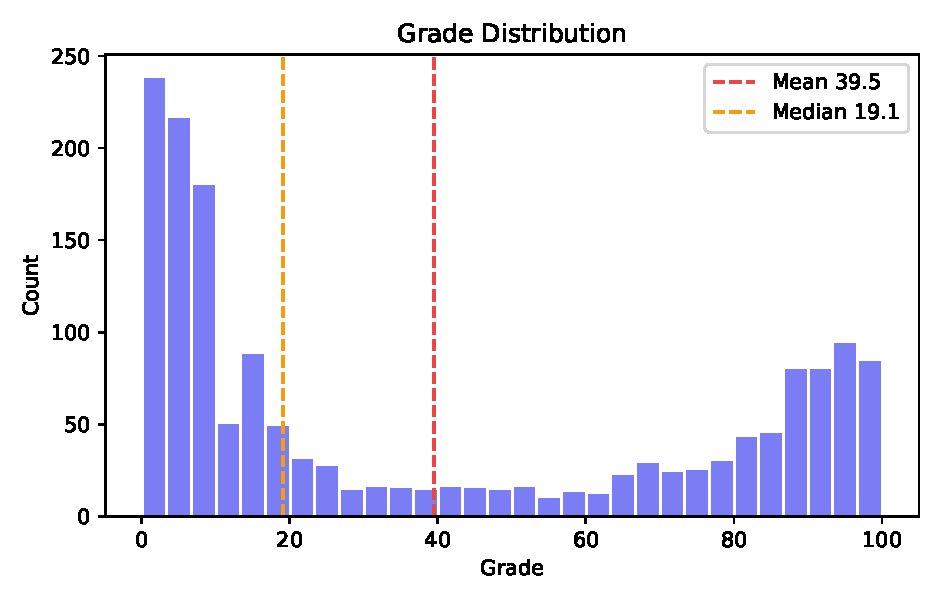
\includegraphics[width=0.82\textwidth]{grade_distribution.pdf}
\caption{学生成绩分布直方图}
\label{fig:grade_dist}
\end{figure}

\subsection{行为特征统计}

表\ref{tab:desc_stats}展示了七个行为特征的描述性统计量。图\ref{fig:boxplot}为标准化后的箱线图。

\begin{table}[H]
\centering
\caption{行为特征描述性统计}
\label{tab:desc_stats}
\begin{tabular}{lrrrrrr}
\toprule
\textbf{特征} & \textbf{均值} & \textbf{中位数} & \textbf{标准差} & \textbf{最小值} & \textbf{最大值} \\
\midrule
在线时长 (s)    & 6,383,131 & 7,265,358 & 3,281,249 & 5       & 10,558,690 \\
活跃天数        & 79.13     & 88.45     & 39.75     & 0       & 151        \\
页面浏览        & 596.62    & 426.00    & 557.46    & 12      & 4,926      \\
课件浏览        & 69.85     & 50.00     & 78.15     & 0       & 1,299      \\
视频观看        & 1,519.00  & 450.00    & 4,766.20  & 0       & 150,372    \\
发帖数          & 0.81      & 0.00      & 3.54      & 0       & 58         \\
评论数          & 0.25      & 0.00      & 1.37      & 0       & 29         \\
\bottomrule
\end{tabular}
\end{table}

可以观察到：（1）在线时长的中位数高于均值，存在一定的左偏；（2）视频观看次数的标准差极大，表明学生之间的视频学习行为差异悬殊；（3）论坛发帖和评论的中位数均为0，说明大多数学生并不参与论坛讨论。

\begin{figure}[H]
\centering
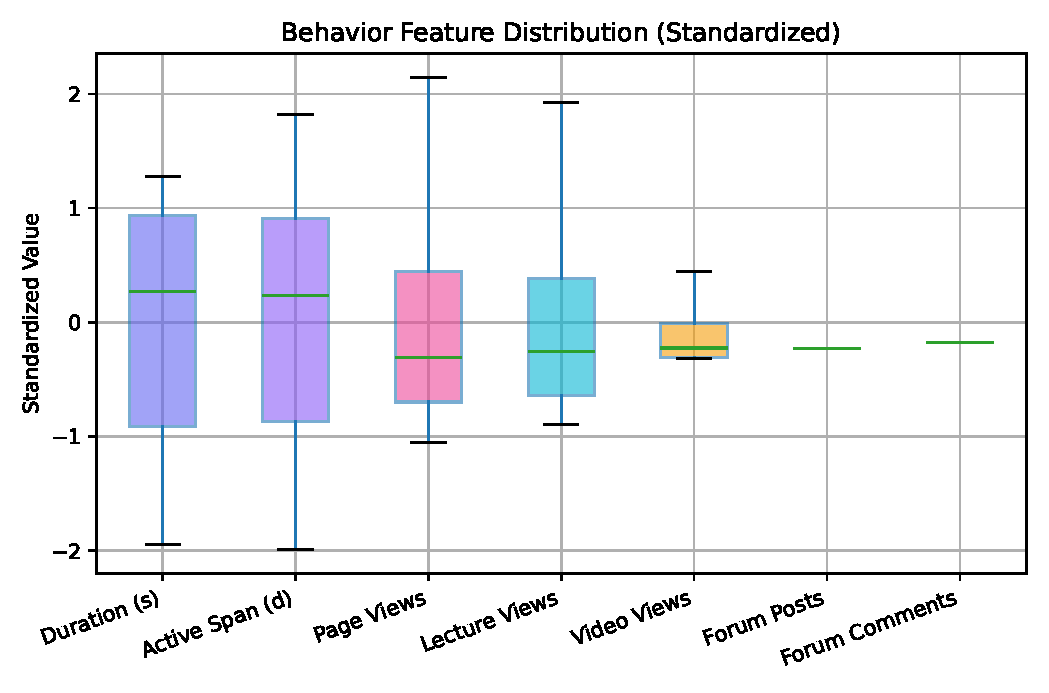
\includegraphics[width=0.85\textwidth]{boxplot_features.pdf}
\caption{行为特征箱线图（标准化后）}
\label{fig:boxplot}
\end{figure}

% ══════════════════════════════════════════════════════════════════════════
\section{相关性分析}
% ══════════════════════════════════════════════════════════════════════════

\subsection{Pearson相关系数矩阵}

图\ref{fig:corr_heatmap}展示了行为特征及成绩之间的Pearson相关系数矩阵。与成绩相关性最强的三个特征分别为：
\begin{itemize}
    \item \textbf{在线时长}（$r = 0.712$）：在线停留时间越长，成绩越高；
    \item \textbf{活跃天数}（$r = 0.703$）：持续学习的时间跨度与成绩正相关；
    \item \textbf{页面浏览}（$r = 0.676$）：浏览更多课程页面的学生成绩更好。
\end{itemize}

论坛参与相关特征（发帖数 $r=0.179$，评论数 $r=0.155$）与成绩的相关性较弱，可能由于大多数学生并不活跃于论坛。

\begin{figure}[H]
\centering
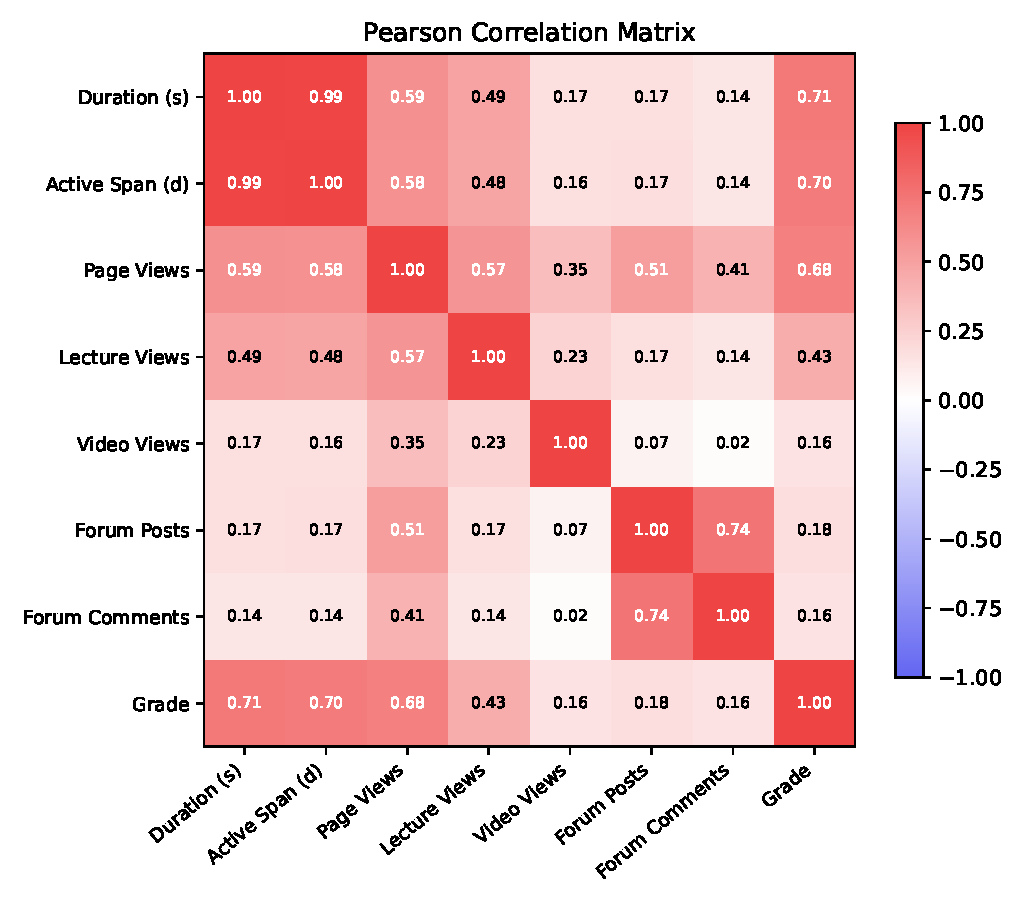
\includegraphics[width=0.78\textwidth]{correlation_heatmap.pdf}
\caption{Pearson 相关系数热力图}
\label{fig:corr_heatmap}
\end{figure}

\subsection{散点图分析}

图\ref{fig:scatter}展示了四个关键行为特征与成绩的散点图。页面浏览和在线时长与成绩呈现较为明显的正相关趋势，但存在较大的离散度，表明行为特征与成绩之间的关系并非简单的线性关系。

\begin{figure}[H]
\centering
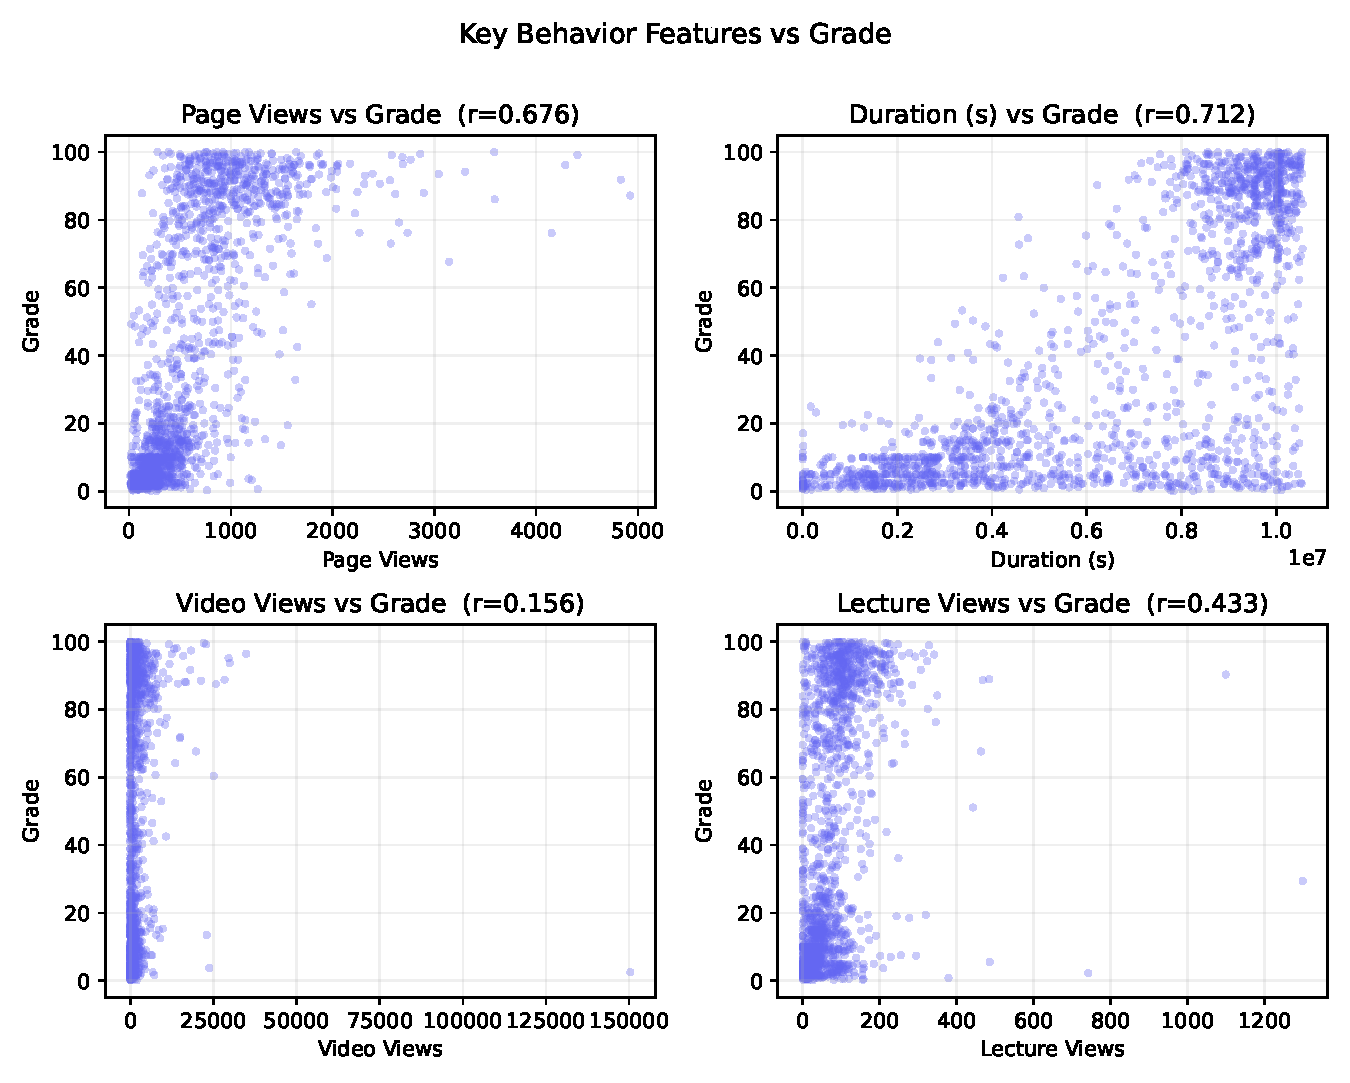
\includegraphics[width=0.92\textwidth]{scatter_top4.pdf}
\caption{关键行为特征与成绩的散点图}
\label{fig:scatter}
\end{figure}

% ══════════════════════════════════════════════════════════════════════════
\section{聚类分析}
% ══════════════════════════════════════════════════════════════════════════

\subsection{最优K值选取}

采用K-Means聚类算法，对标准化后的七个行为特征进行聚类。图\ref{fig:elbow}同时展示了肘部法则（Inertia曲线）和轮廓系数（Silhouette Score）随聚类数$K$的变化。

轮廓系数在$K=3$时取得最大值0.449，表明三类划分最为合理。

\begin{figure}[H]
\centering
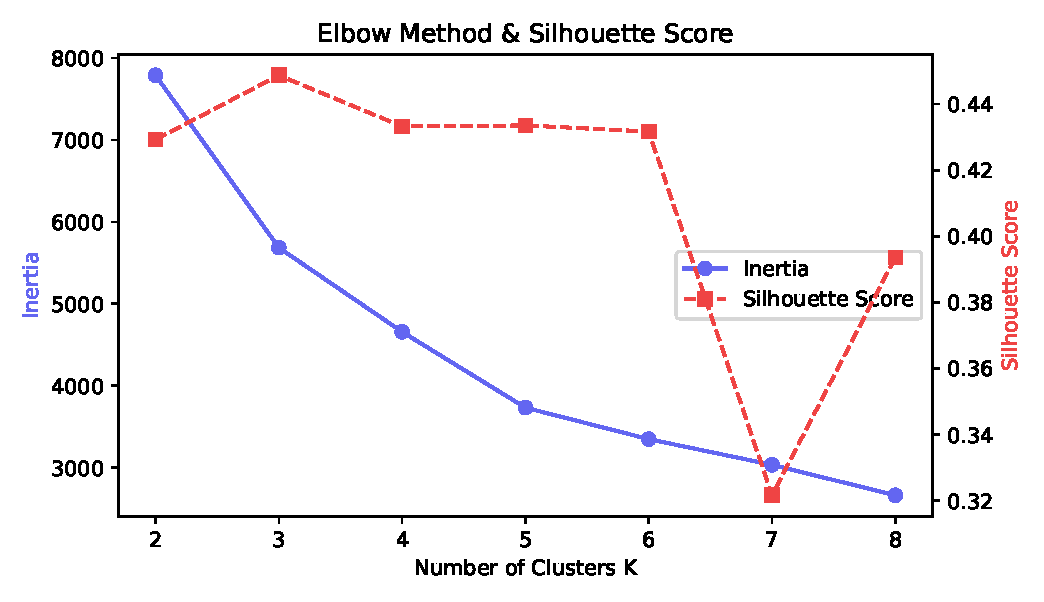
\includegraphics[width=0.82\textwidth]{elbow_silhouette.pdf}
\caption{肘部法则与轮廓系数}
\label{fig:elbow}
\end{figure}

\subsection{聚类结果可视化}

图\ref{fig:pca}展示了$K=3$时的PCA降维聚类散点图。三个簇在二维空间中有较好的分离度。

\begin{figure}[H]
\centering
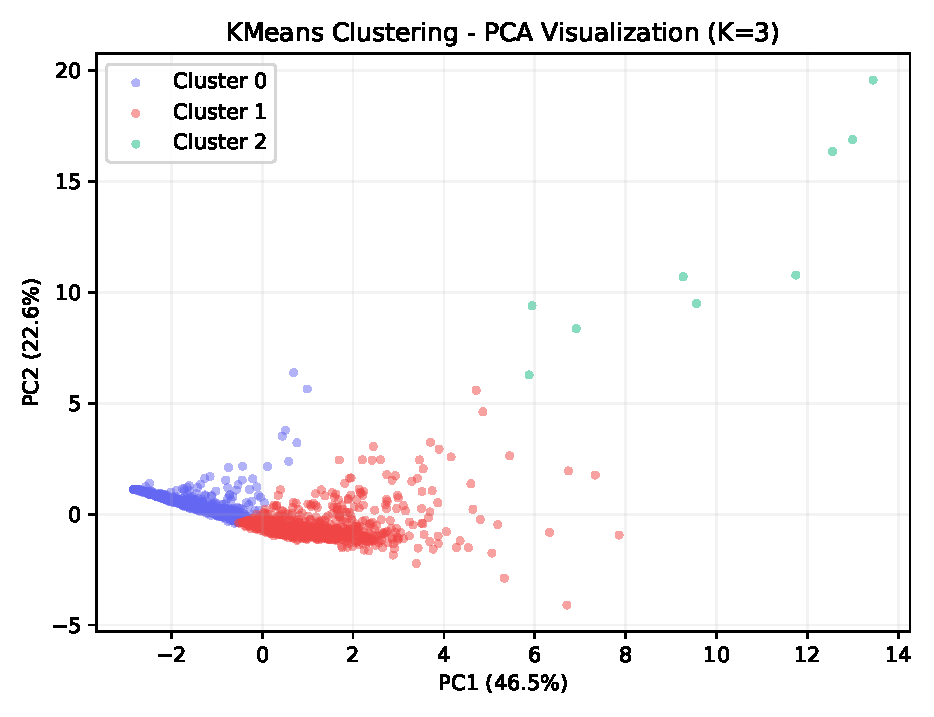
\includegraphics[width=0.78\textwidth]{cluster_pca.pdf}
\caption{KMeans聚类的PCA降维可视化（$K=3$）}
\label{fig:pca}
\end{figure}

\subsection{各簇特征对比}

表\ref{tab:cluster}和图\ref{fig:radar}分别以数值和雷达图的形式展示了三个簇的行为特征差异。

\begin{table}[H]
\centering
\caption{三个聚类簇的基本统计}
\label{tab:cluster}
\begin{tabular}{lrrr}
\toprule
 & \textbf{簇 0} & \textbf{簇 1} & \textbf{簇 2} \\
\midrule
样本数   & 736   & 875   & 9     \\
平均成绩 & 11.89 & 62.18 & 88.57 \\
\bottomrule
\end{tabular}
\end{table}

\begin{itemize}
    \item \textbf{簇 0}（低活跃-低成绩组）：736人，平均成绩仅11.89分，各行为指标均偏低。
    \item \textbf{簇 1}（中高活跃-中高成绩组）：875人，平均成绩62.18分，学习行为较为活跃。
    \item \textbf{簇 2}（极高活跃-高成绩组）：9人，平均成绩88.57分，属于学习极为投入的少数学生。
\end{itemize}

\begin{figure}[H]
\centering
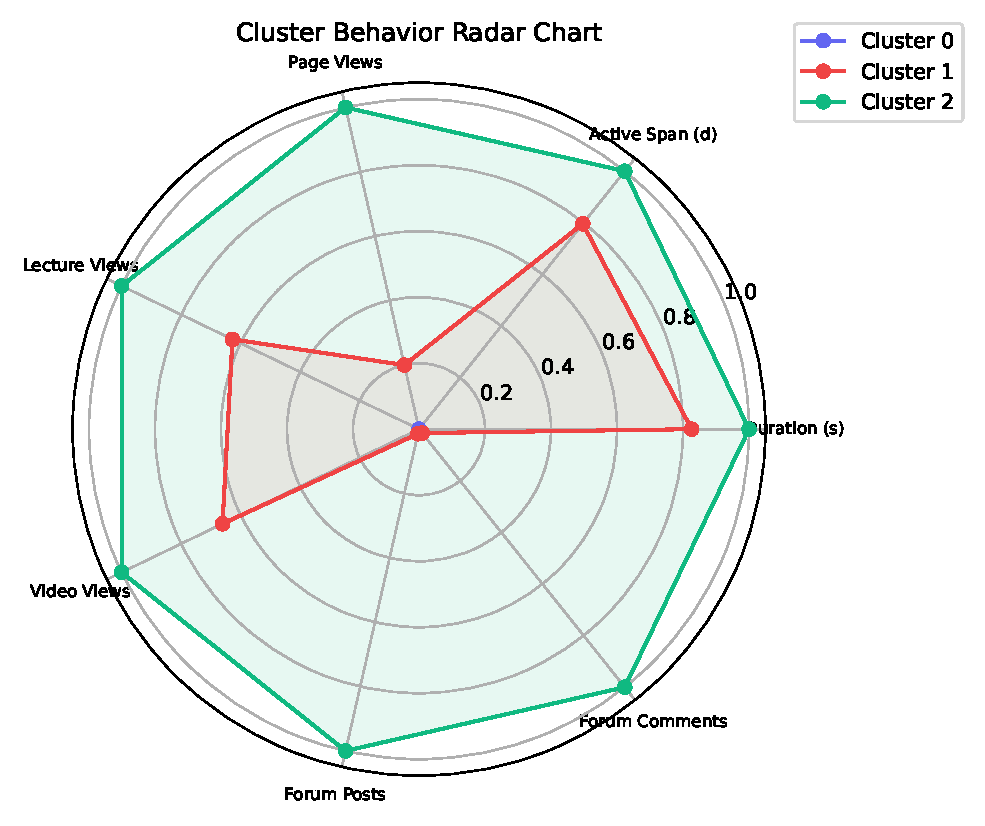
\includegraphics[width=0.7\textwidth]{cluster_radar.pdf}
\caption{各簇行为特征雷达图（归一化）}
\label{fig:radar}
\end{figure}

% ══════════════════════════════════════════════════════════════════════════
\section{回归分析}
% ══════════════════════════════════════════════════════════════════════════

\subsection{线性回归模型}

以七个行为特征作为自变量、成绩作为因变量，构建线性回归模型。模型在测试集上的评估指标如表\ref{tab:reg_metrics}所示。

\begin{table}[H]
\centering
\caption{线性回归模型评估指标}
\label{tab:reg_metrics}
\begin{tabular}{lr}
\toprule
\textbf{指标} & \textbf{值} \\
\midrule
$R^2$（决定系数）       & 0.6140 \\
MSE（均方误差）         & 550.68 \\
MAE（平均绝对误差）     & 18.25  \\
\bottomrule
\end{tabular}
\end{table}

$R^2 = 0.614$表明仅使用行为特征即可解释成绩方差的61.4\%，说明学习行为对成绩有较强的预测能力，但仍有约38.6\%的方差无法由当前特征解释，可能与学生的先验知识、学习能力等不可观测因素有关。

\subsection{预测效果可视化}

图\ref{fig:reg_pred}展示了实际成绩与预测成绩的对比散点图。理想预测应落在对角线上。可以看到模型在中高分段的预测较为准确，但在低分段存在一定的过估。

\begin{figure}[H]
\centering
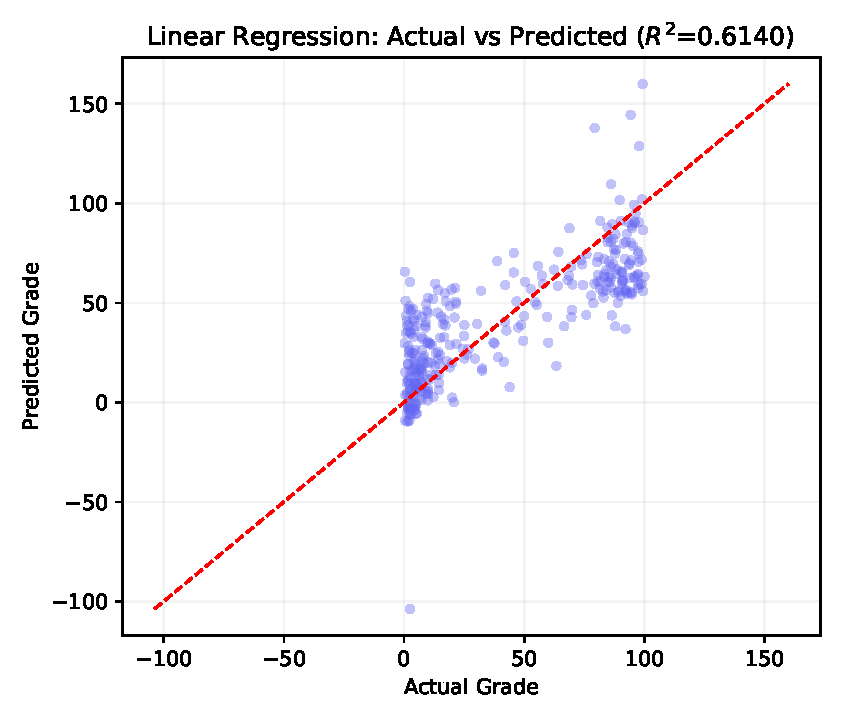
\includegraphics[width=0.72\textwidth]{regression_actual_vs_pred.pdf}
\caption{线性回归：实际成绩 vs 预测成绩}
\label{fig:reg_pred}
\end{figure}

图\ref{fig:residual}展示了残差的分布。残差整体呈近似正态分布，均值接近0，说明模型没有系统性偏差。

\begin{figure}[H]
\centering
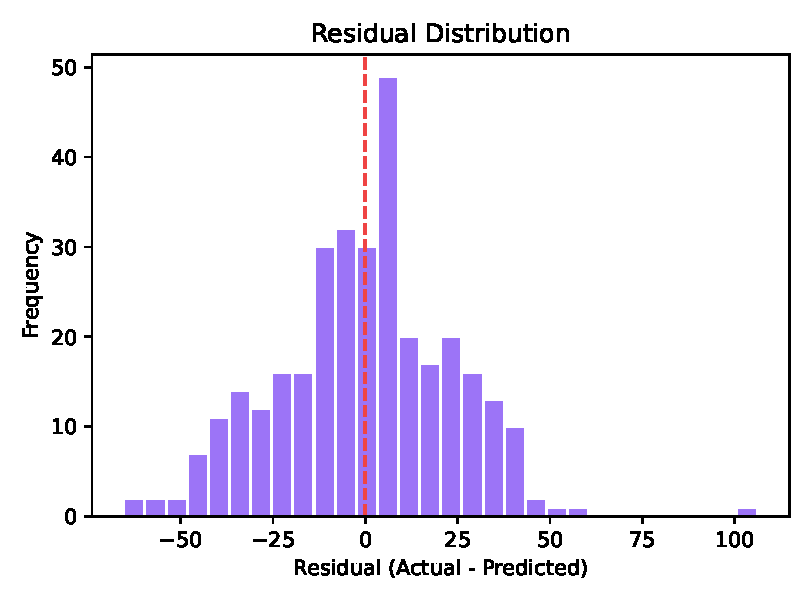
\includegraphics[width=0.72\textwidth]{regression_residual.pdf}
\caption{残差分布}
\label{fig:residual}
\end{figure}

% ══════════════════════════════════════════════════════════════════════════
\section{分类预测}
% ══════════════════════════════════════════════════════════════════════════

\subsection{分类任务设定}

以成绩中位数（19.06分）为阈值，将学生分为``高分组''（$\geq$中位数）和``低分组''（$<$中位数），构建二分类模型。

\subsection{模型对比}

表\ref{tab:cls}展示了三种分类模型的性能对比。

\begin{table}[H]
\centering
\caption{分类模型性能对比}
\label{tab:cls}
\begin{tabular}{lcccc}
\toprule
\textbf{模型} & \textbf{Accuracy} & \textbf{Precision} & \textbf{Recall} & \textbf{F1 Score} \\
\midrule
逻辑回归     & 0.8210 & --- & --- & 0.8232 \\
决策树       & 0.8426 & --- & --- & 0.8381 \\
MLP神经网络  & 0.8457 & --- & --- & 0.8457 \\
\bottomrule
\end{tabular}
\end{table}

\begin{figure}[H]
\centering
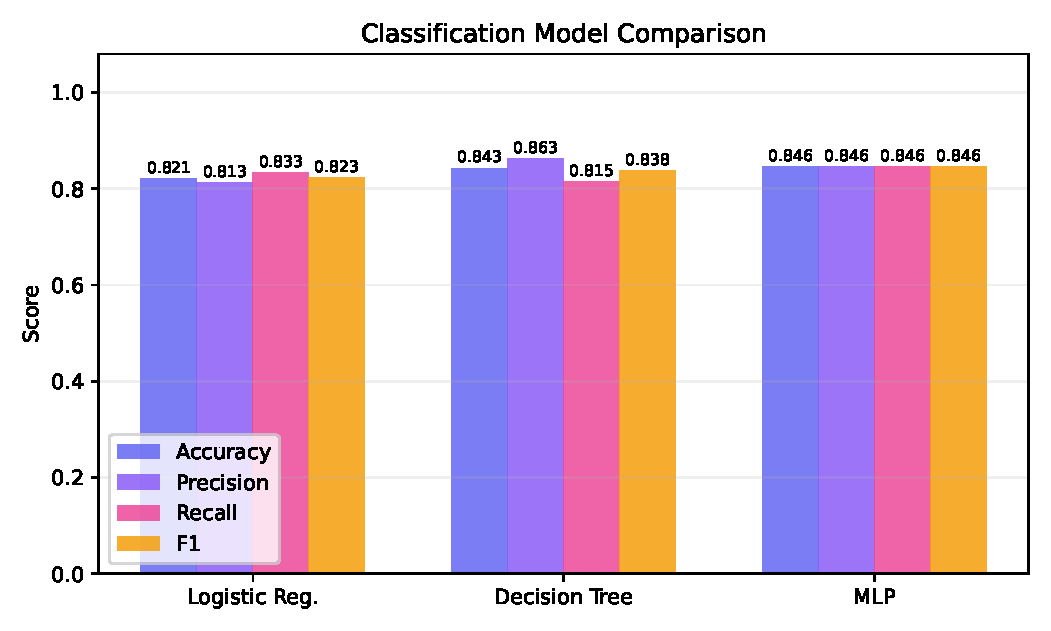
\includegraphics[width=0.88\textwidth]{classification_comparison.pdf}
\caption{三种分类模型性能对比}
\label{fig:cls_compare}
\end{figure}

三种模型的准确率均超过82\%。MLP神经网络以84.57\%的准确率和0.846的F1值取得最佳表现，但与决策树（84.26\%）差距不大。考虑到决策树的可解释性更强，在实际应用中两者均为可行选择。

\subsection{混淆矩阵分析}

图\ref{fig:confusion}展示了三种模型的混淆矩阵。

\begin{figure}[H]
\centering
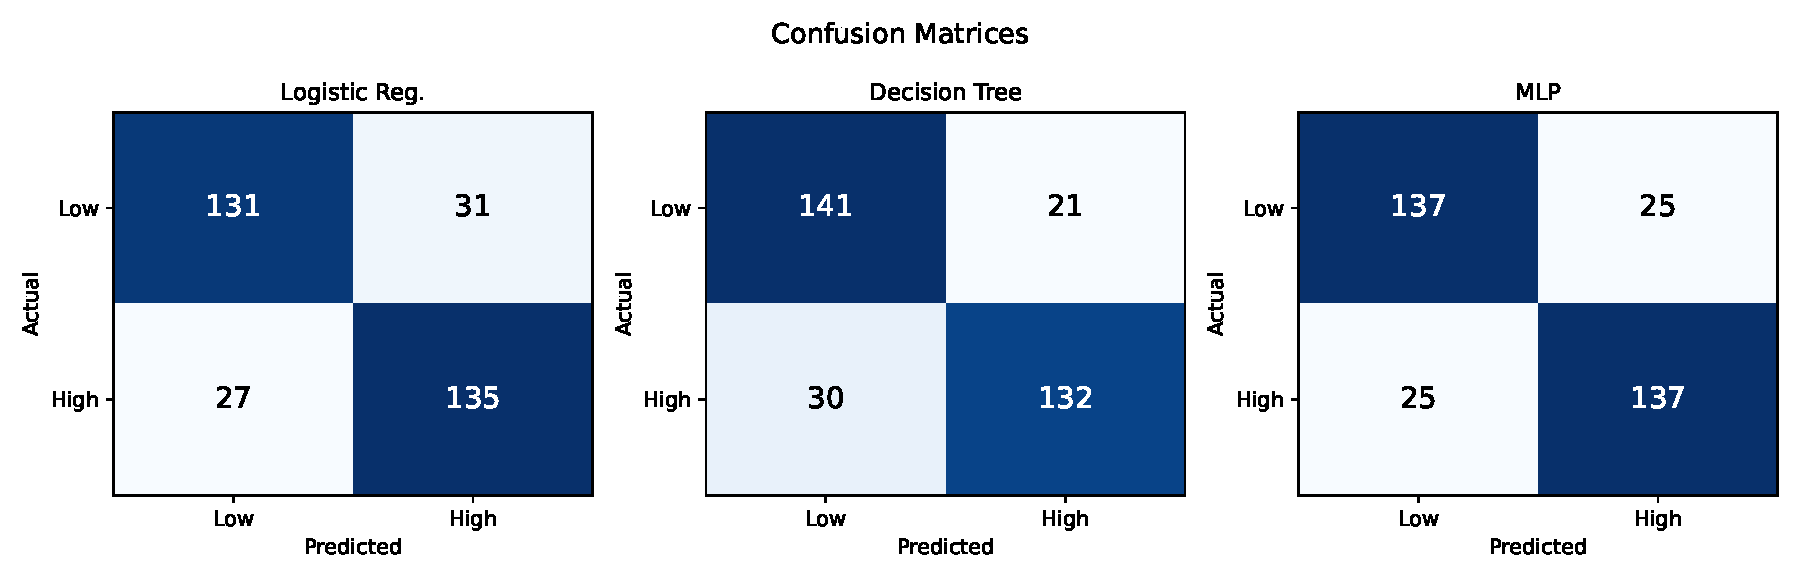
\includegraphics[width=0.95\textwidth]{confusion_matrices.pdf}
\caption{三种模型的混淆矩阵}
\label{fig:confusion}
\end{figure}

% ══════════════════════════════════════════════════════════════════════════
\section{分组分析}
% ══════════════════════════════════════════════════════════════════════════

\subsection{地区差异}

图\ref{fig:region}展示了不同地区学生的平均成绩对比。由于数据集以美洲地区（特别是北美）学生为主，地区间的样本量差异较大，需要谨慎解读。

\begin{figure}[H]
\centering
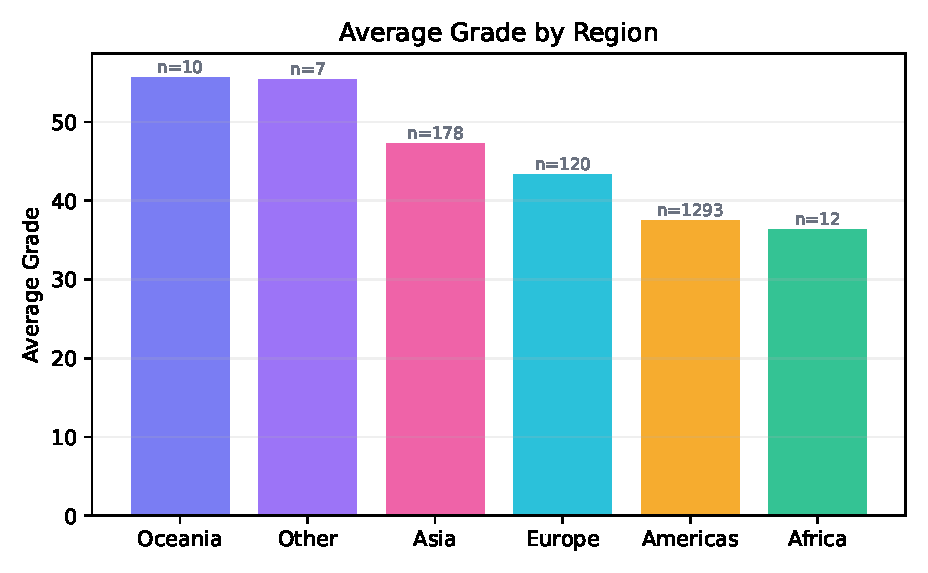
\includegraphics[width=0.78\textwidth]{region_grade.pdf}
\caption{不同地区学生平均成绩对比}
\label{fig:region}
\end{figure}

\subsection{活跃天数与成绩}

图\ref{fig:span}展示了不同活跃天数分箱下的平均成绩和学生人数。活跃天数越长的学生，平均成绩越高，进一步验证了持续学习对成绩的正向影响。

\begin{figure}[H]
\centering
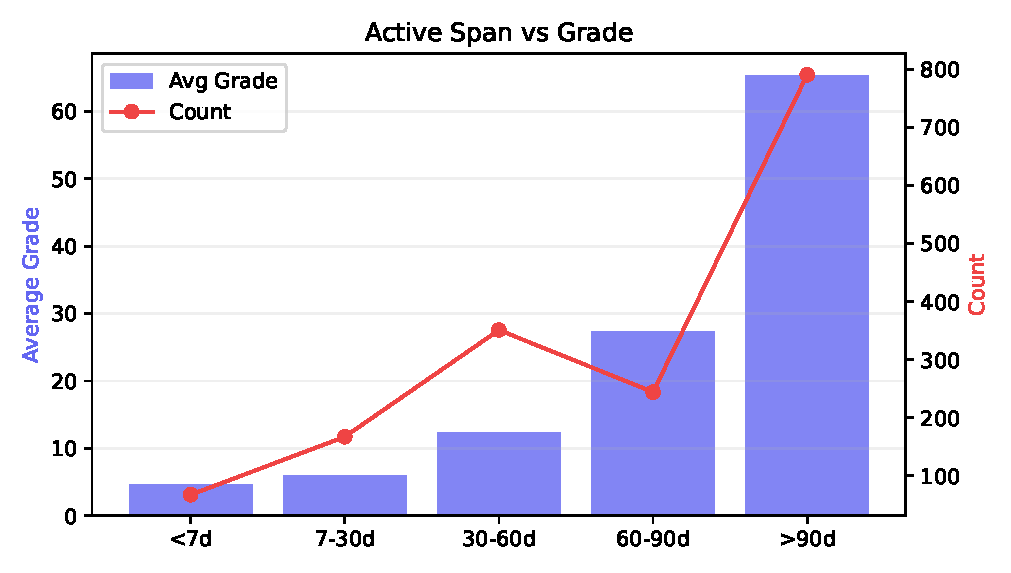
\includegraphics[width=0.78\textwidth]{span_grade.pdf}
\caption{活跃天数分箱与成绩关系}
\label{fig:span}
\end{figure}

% ══════════════════════════════════════════════════════════════════════════
\section{在线分析平台 EduAnalytics}
% ══════════════════════════════════════════════════════════════════════════

为了让前述分析方法不仅停留在离线脚本的形式，本文还开发了一个配套的交互式可视化与AI问答平台——\textbf{EduAnalytics}。该平台整合了数据上传、自动分析、交互可视化与大语言模型问答四类能力，面向教师、助教和课程研究者，显著降低了对同类数据集进行探索性分析的门槛。平台整体界面见图\ref{fig:platform_home}。

\medskip
\noindent\textbf{开源地址：} 平台源码已公开发布于 GitHub，仓库地址为\\ \url{https://github.com/Lee-Eee-Eee/EduAnalytics}，读者可自行克隆并部署到本地环境中运行。

\medskip
\noindent\textbf{在线访问：} 平台同步部署于 Render 云服务，读者无需本地安装即可通过浏览器直接体验全部功能：\\ \url{https://eduanalytics-qpq7.onrender.com/}（Render 免费实例首次访问可能存在约 30 秒的冷启动延迟）。

\begin{figure}[H]
\centering
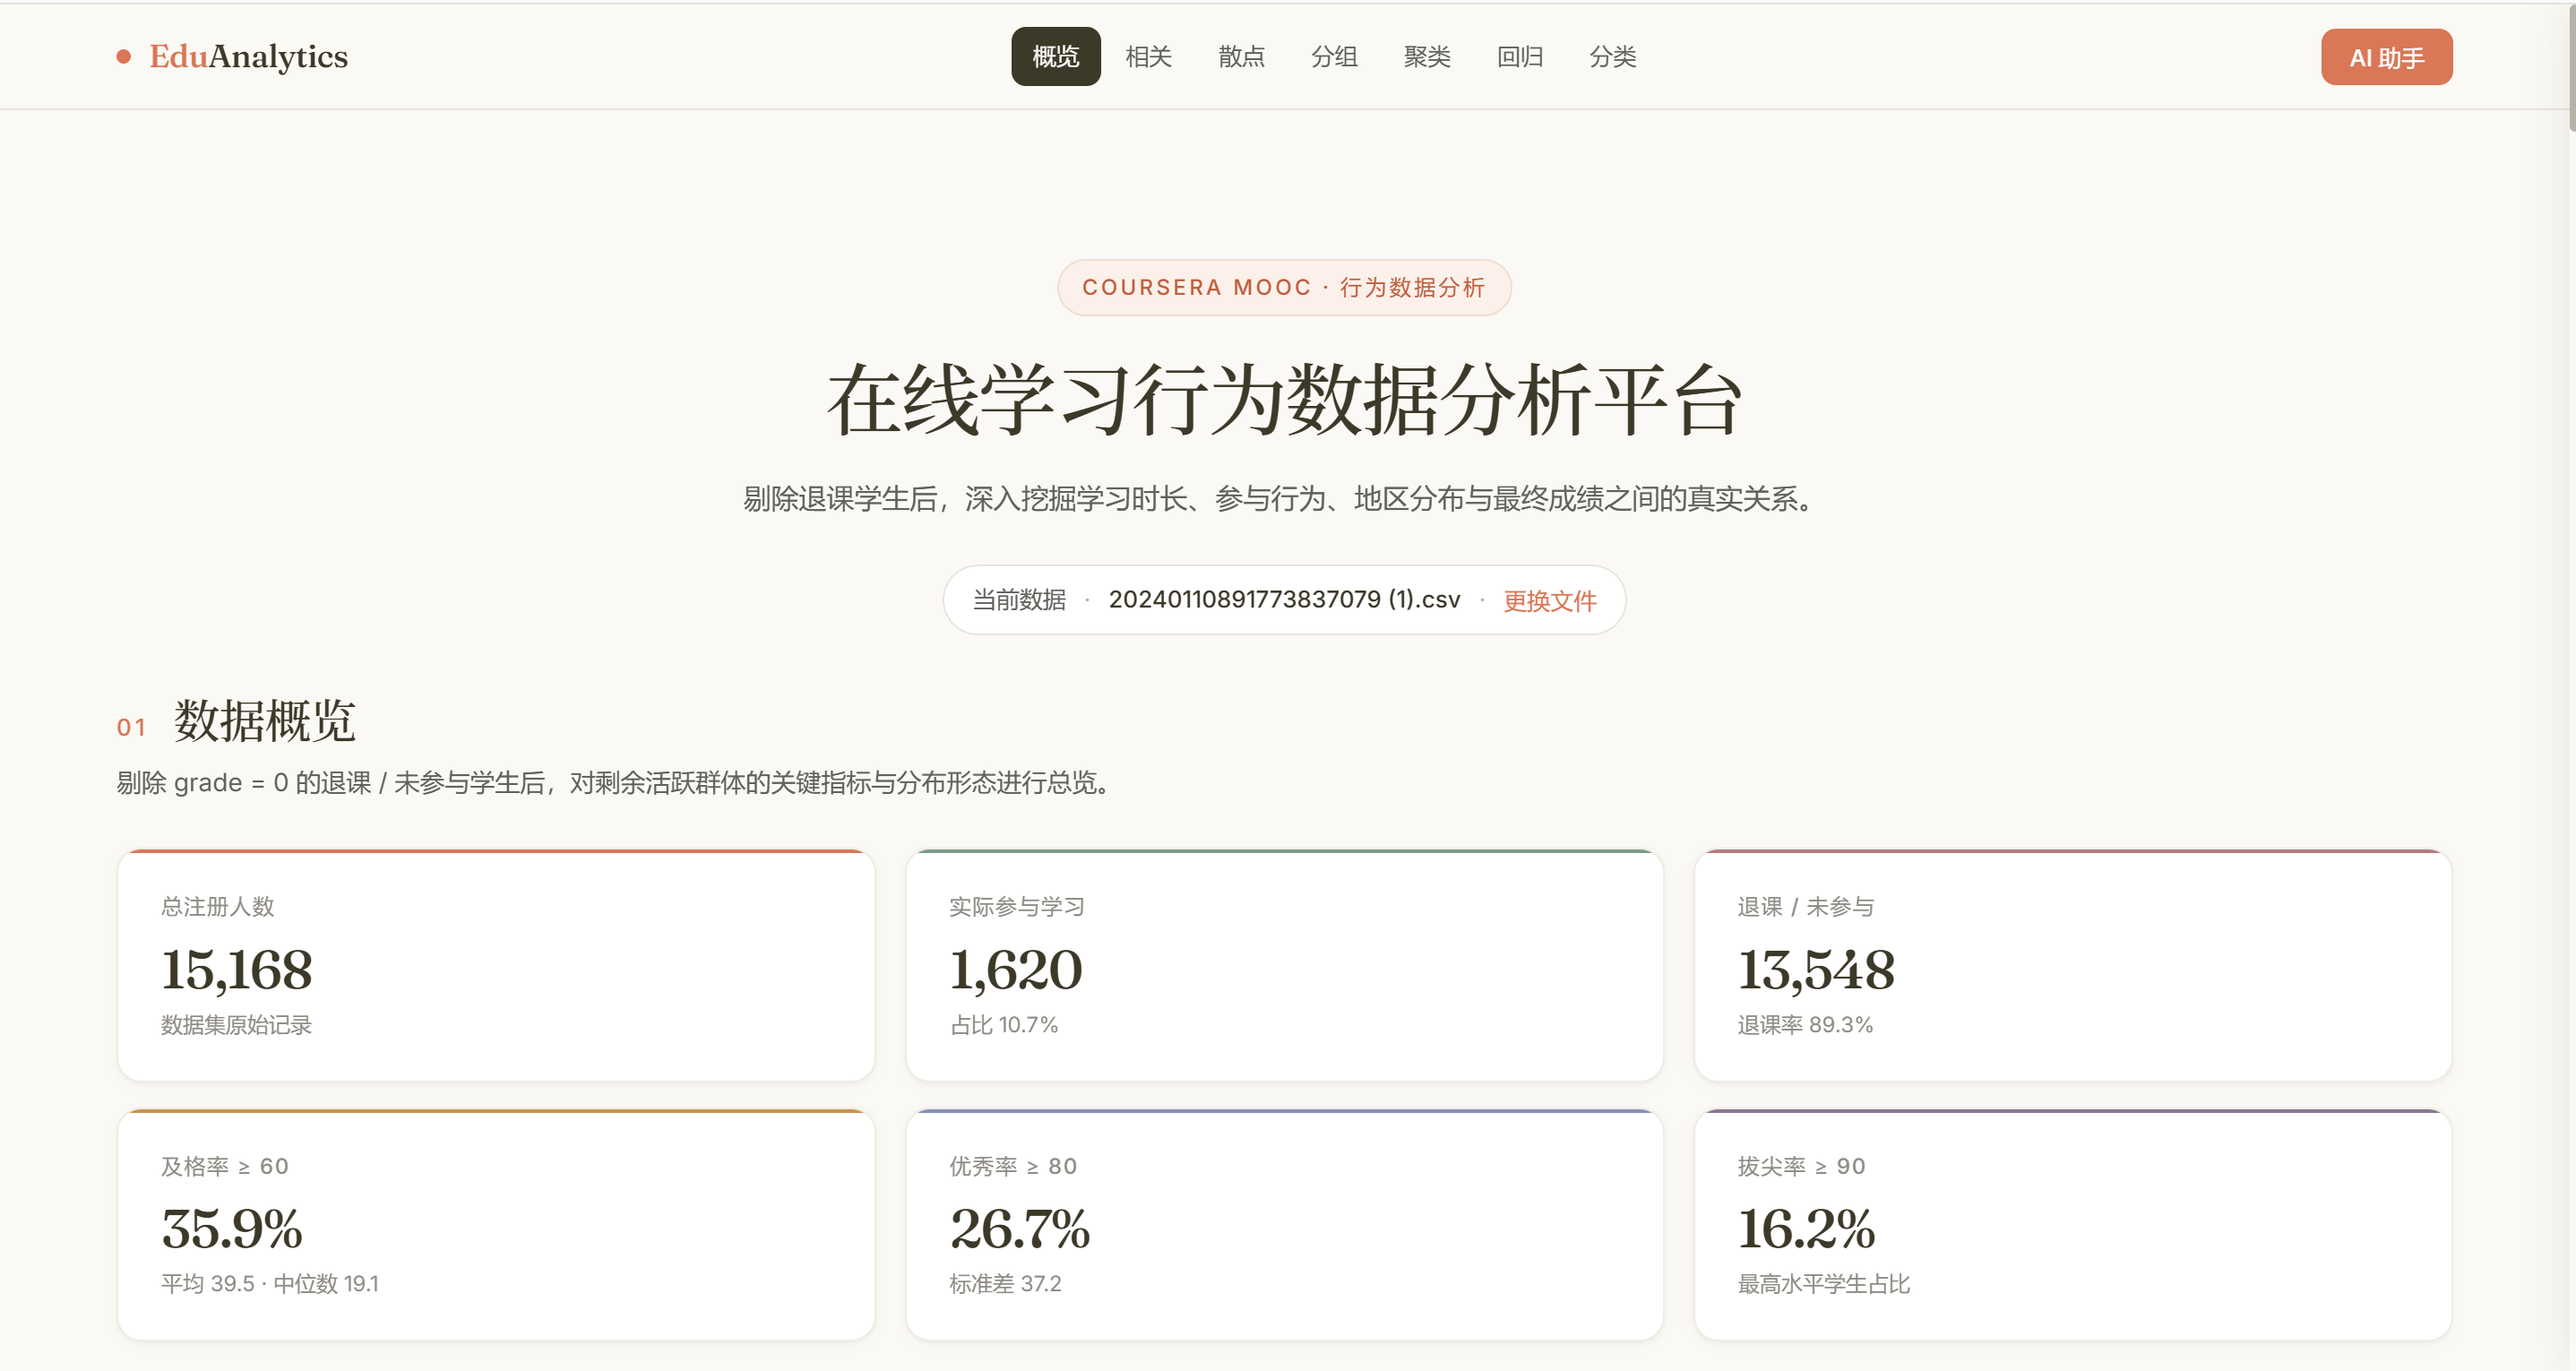
\includegraphics[width=0.96\textwidth]{platform.png}
\caption{EduAnalytics 平台主界面：英雄区与数据概览卡片}
\label{fig:platform_home}
\end{figure}

\subsection{平台定位与目标}

平台的设计目标包括：
\begin{itemize}
    \item \textbf{轻量部署}：后端基于Flask，无需额外数据库或中间件；借助\texttt{uv sync}一条命令即可还原与开发环境完全一致的依赖版本，避免手动处理版本冲突；
    \item \textbf{一键分析}：服务启动后，通过浏览器拖拽上传CSV文件即可自动完成本文所涉及的描述性统计、相关性分析、聚类、回归与分类等全流程计算；
    \item \textbf{可交互探索}：所有图表均支持悬停、缩放、筛选等交互操作，替代静态图片的表达方式；
    \item \textbf{数据感知的AI问答}：集成LLM对话模块，在每次提问时自动附加当前数据集的关键统计信息，实现“先算后聊”的闭环。
\end{itemize}

\subsection{系统架构}

平台采用前后端一体化的轻量级架构，技术栈如表\ref{tab:stack}所示。
\begin{table}[H]
\centering
\caption{EduAnalytics 技术栈}
\label{tab:stack}
\begin{tabular}{lll}
\toprule
\textbf{模块} & \textbf{技术} & \textbf{职责} \\
\midrule
后端服务        & Flask（Python 3.9） & HTTP路由、文件上传、分析编排 \\
数据分析        & pandas, NumPy       & 数据清洗、派生特征、描述性统计 \\
机器学习        & scikit-learn        & 聚类/回归/分类模型训练与评估 \\
前端框架        & 原生 HTML + JavaScript & 交互式界面与状态管理 \\
可视化          & Apache ECharts 5    & 热力图、散点图、箱线图、雷达图等 \\
AI 对话         & LLM 兼容代理         & 流式转发聊天请求并注入系统提示词 \\
\bottomrule
\end{tabular}
\end{table}

整体数据流如下：
\begin{enumerate}
    \item 用户通过浏览器拖拽或点击上传CSV至 \texttt{/api/upload} 接口；
    \item 后端调用 \texttt{prepare\_dataframe()} 完成派生字段计算（\texttt{active\_span}、\texttt{region}等）与退课学生剔除；
    \item 随后按序调用七个分析函数：\texttt{compute\_overview}、\texttt{compute\_correlation}、\texttt{compute\_scatter}、\texttt{compute\_group\_analysis}、\texttt{compute\_clustering}、\texttt{compute\_regression}、\texttt{compute\_classification}；
    \item 分析结果以JSON形式注入模板，前端使用ECharts即时渲染为7个章节、共计20余个可交互图表；
    \item 用户向AI助手提问时，请求经由 \texttt{/api/chat} 代理至第三方LLM服务，系统自动附加包含数据概况、相关性、分组统计和样本行的上下文。
\end{enumerate}

\subsection{界面与功能模块}

平台的界面采用\textbf{暖色米白配色}与\textbf{Fraunces 衬线标题字体}，整体风格简洁克制、视觉压力低，便于长时间阅读（见图\ref{fig:platform_detail}）。主体界面划分为顶部固定导航栏、英雄区（数据集信息及更换入口）、以及与前文章节一一对应的\textbf{七个分析章节}；右侧通过滑出式面板承载\textbf{AI 助手}模块。

\begin{figure}[H]
\centering
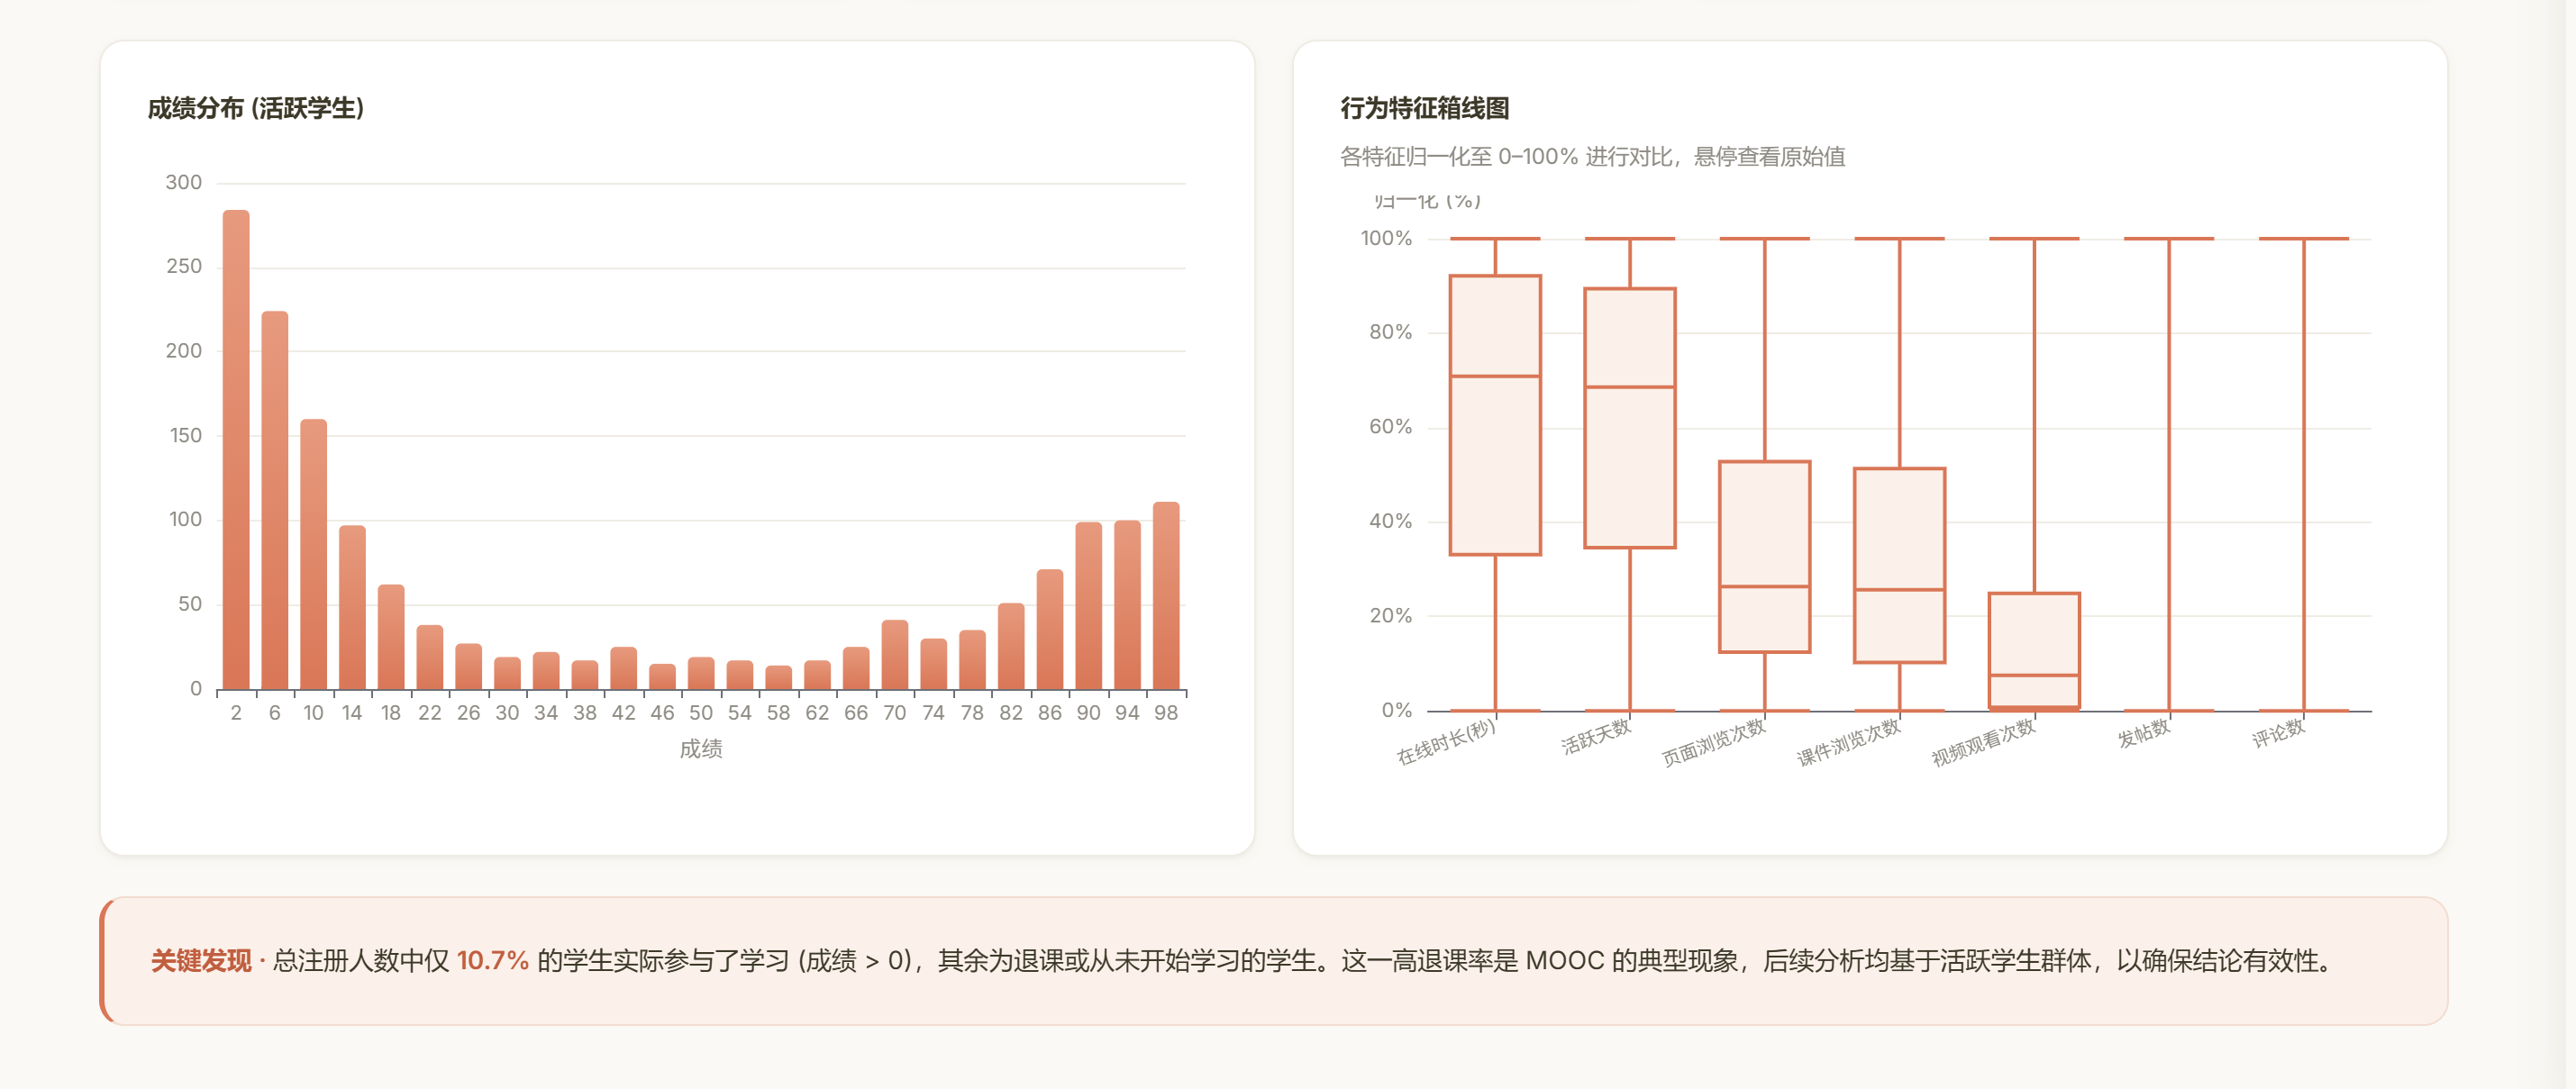
\includegraphics[width=0.96\textwidth]{platform_1.png}
\caption{EduAnalytics 的分析视图：统一的卡片布局与交互式图表}
\label{fig:platform_detail}
\end{figure}

\begin{itemize}
    \item \textbf{上传入口}：首次访问时显示全屏拖拽区域，支持文件选择与拖放两种方式，对非 CSV 文件和缺少 \texttt{grade} 列的数据会给出明确错误提示。
    \item \textbf{数据概览}：以六张卡片展示总注册数、活跃人数、退课率、三率（及格/优秀/拔尖）以及平均成绩等关键指标，配合成绩直方图与行为特征归一化箱线图。
    \item \textbf{相关性分析}：同时提供七阶相关系数热力图与“特征—成绩”相关系数排序条形图，正负相关以不同色调区分（见图\ref{fig:webview_corr}）。
    \item \textbf{散点图}：支持切换 X 轴变量并自动绘制最小二乘拟合线，实时显示相关系数。
    \item \textbf{分组对比}：以“条形 + 折线双轴”的形式同时呈现平均成绩与三率，覆盖地区、账户状态、活跃天数三类分组（见图\ref{fig:webview_region}）。
    \item \textbf{聚类分析}：包含肘部 / 轮廓双指标曲线、PCA 降维散点、各簇统计卡片与特征雷达图（见图\ref{fig:webview_kmeans}）。
    \item \textbf{回归分析}：展示指标卡片（$R^2$、MSE、MAE、截距）、回归系数条形图、预测值对角线图以及残差分布直方图。
    \item \textbf{分类分析}：并列对比三种模型的 Accuracy / Precision / Recall / F1 指标，可切换混淆矩阵并查看决策树的特征重要性（见图\ref{fig:webview_cls}）。
    \item \textbf{AI 助手}：点击右上角按钮呼出侧边栏，支持填写任意 OpenAI 兼容 API（\texttt{base URL}、\texttt{API Key}、模型名）；所填写的凭据通过浏览器 \texttt{localStorage} 持久化，刷新或下次打开时自动恢复，不再需要重复输入。对话过程采用 SSE 流式渲染，并实时解析 Markdown 与代码块。AI 助手在每次请求时自动附加当前数据集的关键统计信息，使其能结合具体数据作答，其对话界面与典型回答示例见图\ref{fig:ai_chat_1}与图\ref{fig:ai_chat_2}。
\end{itemize}

\begin{figure}[H]
\centering
\begin{subfigure}{0.48\textwidth}
    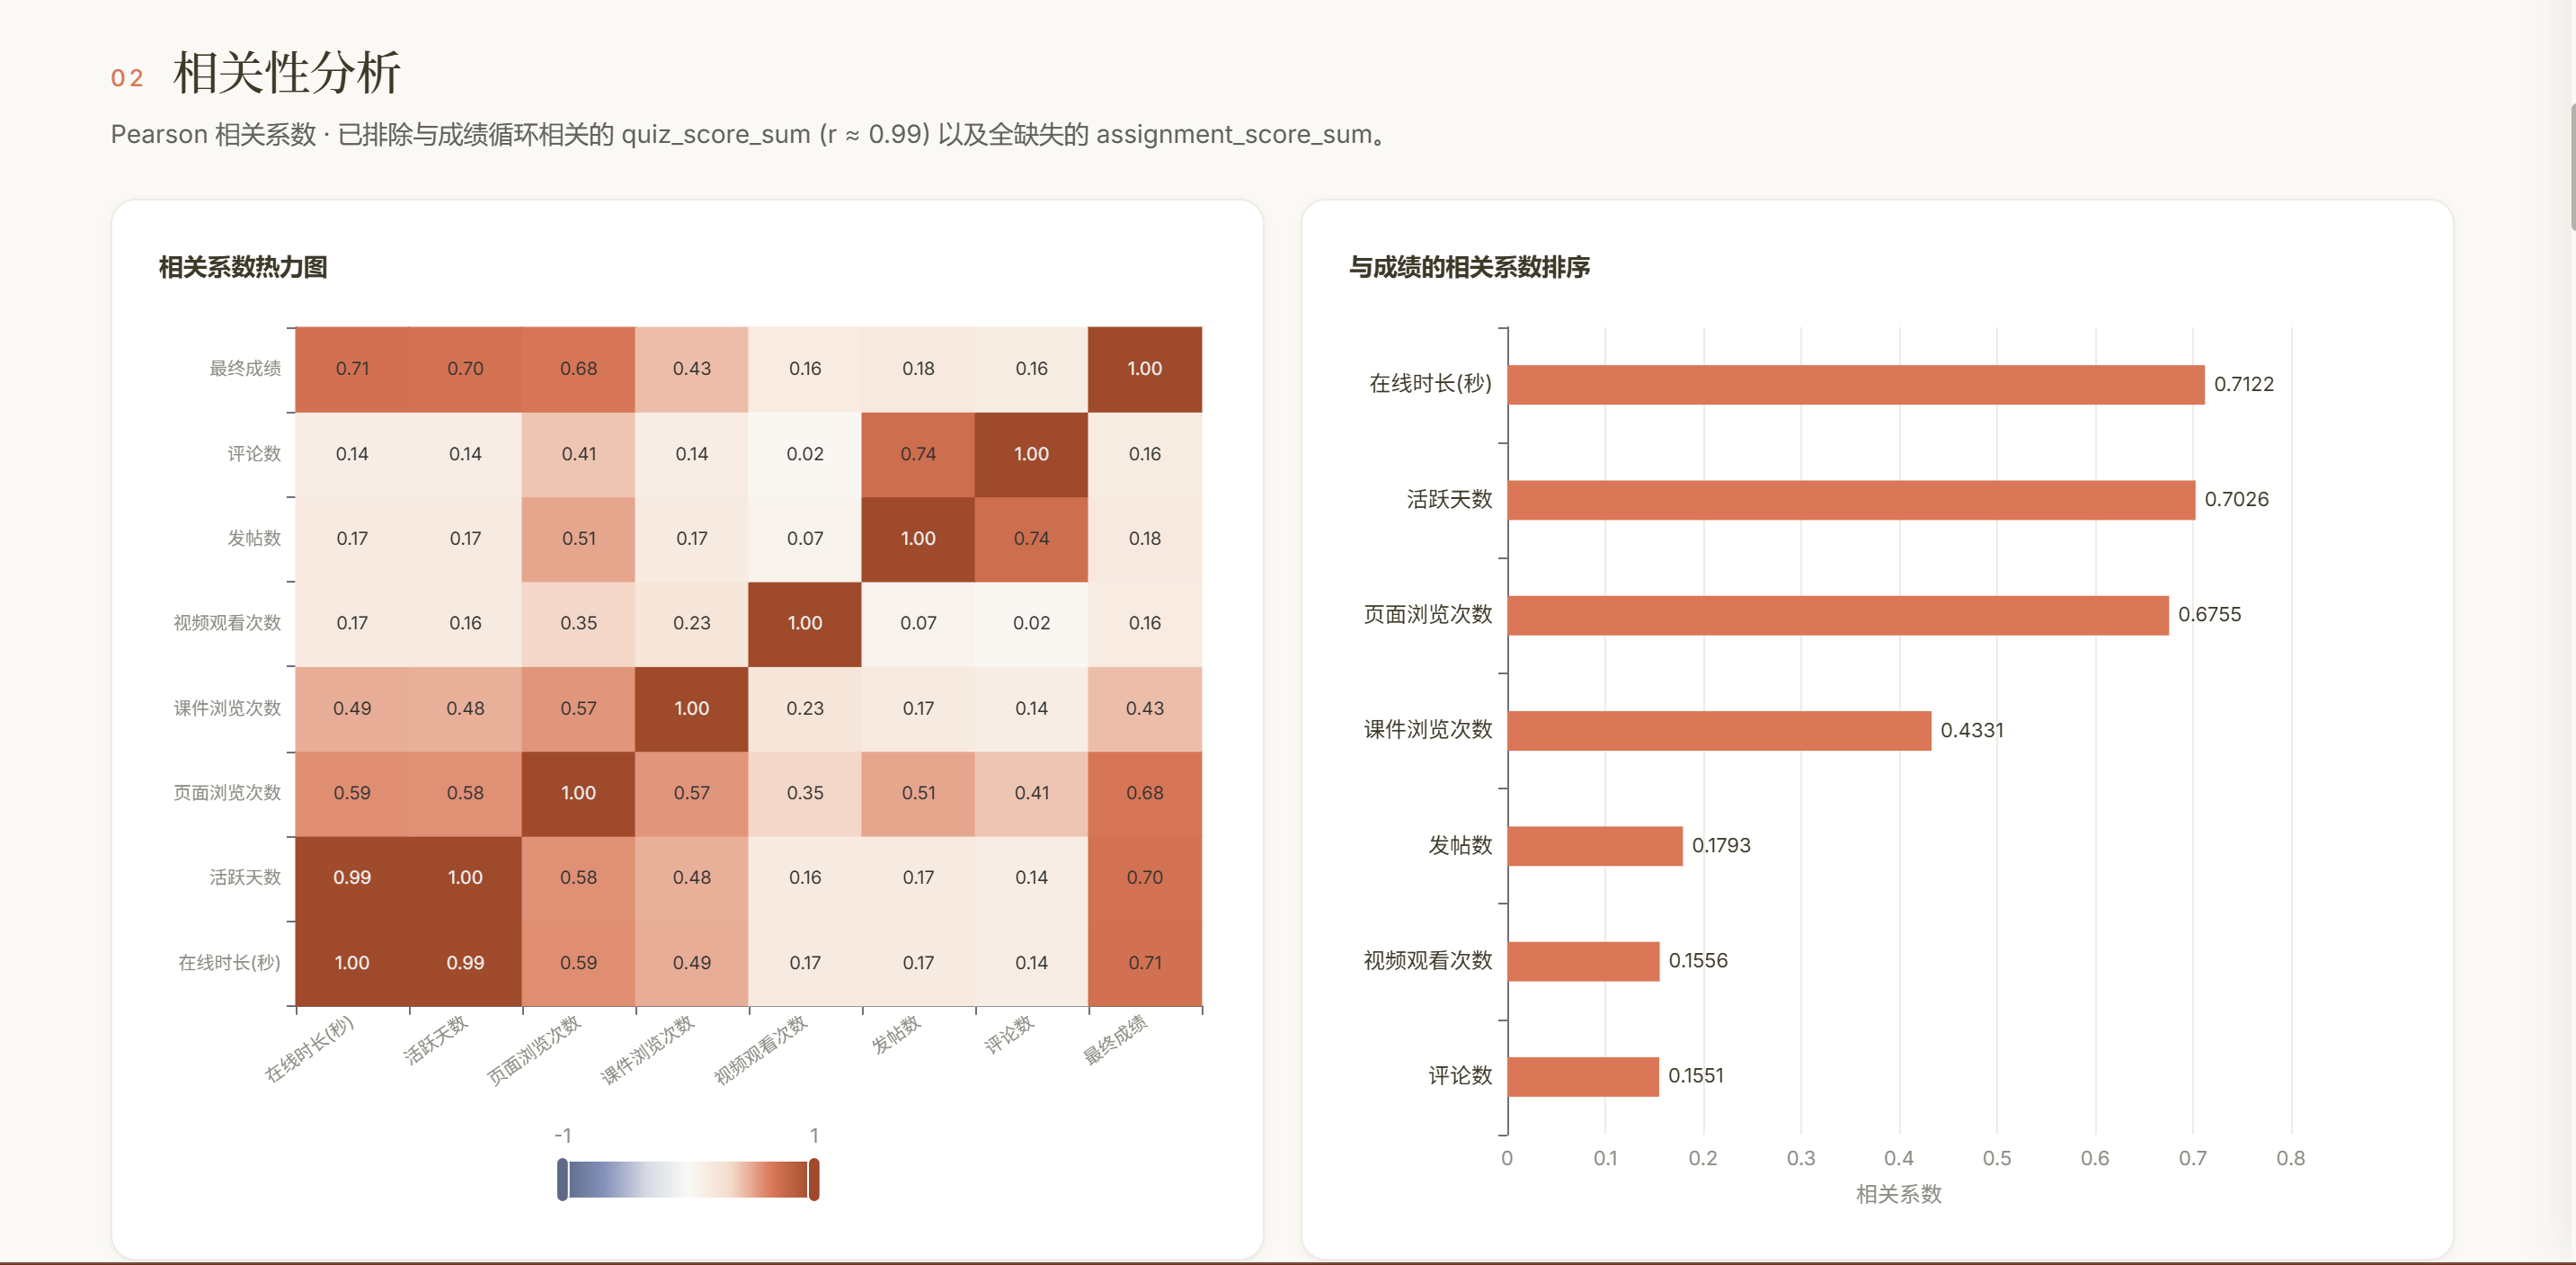
\includegraphics[width=\textwidth]{refrence.png}
    \caption{相关性章节的热力图与条形图}
    \label{fig:webview_corr}
\end{subfigure}\hfill
\begin{subfigure}{0.48\textwidth}
    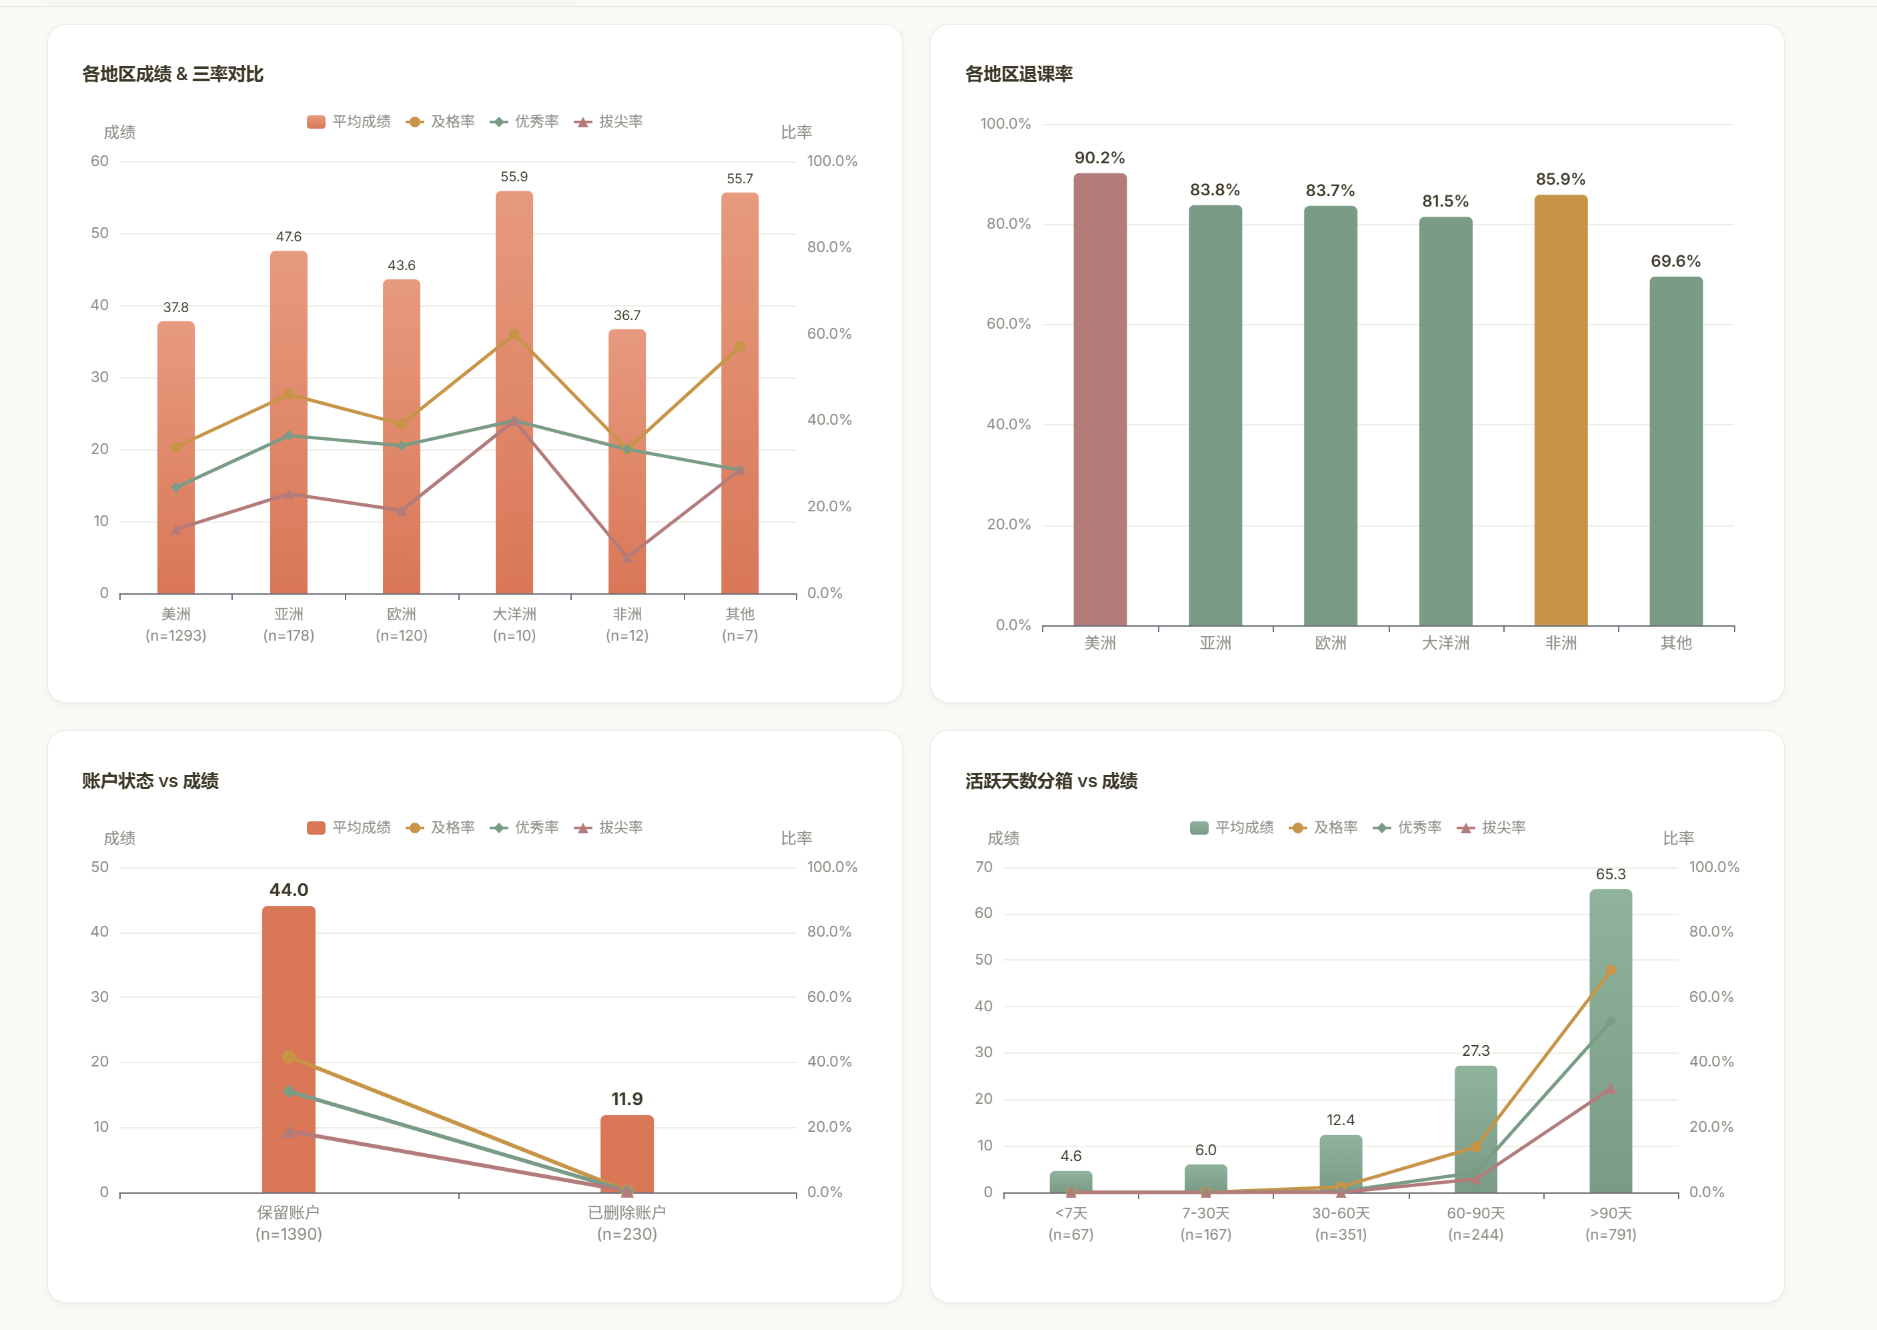
\includegraphics[width=\textwidth]{areas.png}
    \caption{分组对比章节的地区分析}
    \label{fig:webview_region}
\end{subfigure}
\caption{EduAnalytics 相关性与分组分析页面}
\label{fig:webview_analysis1}
\end{figure}

\begin{figure}[H]
\centering
\begin{subfigure}{0.48\textwidth}
    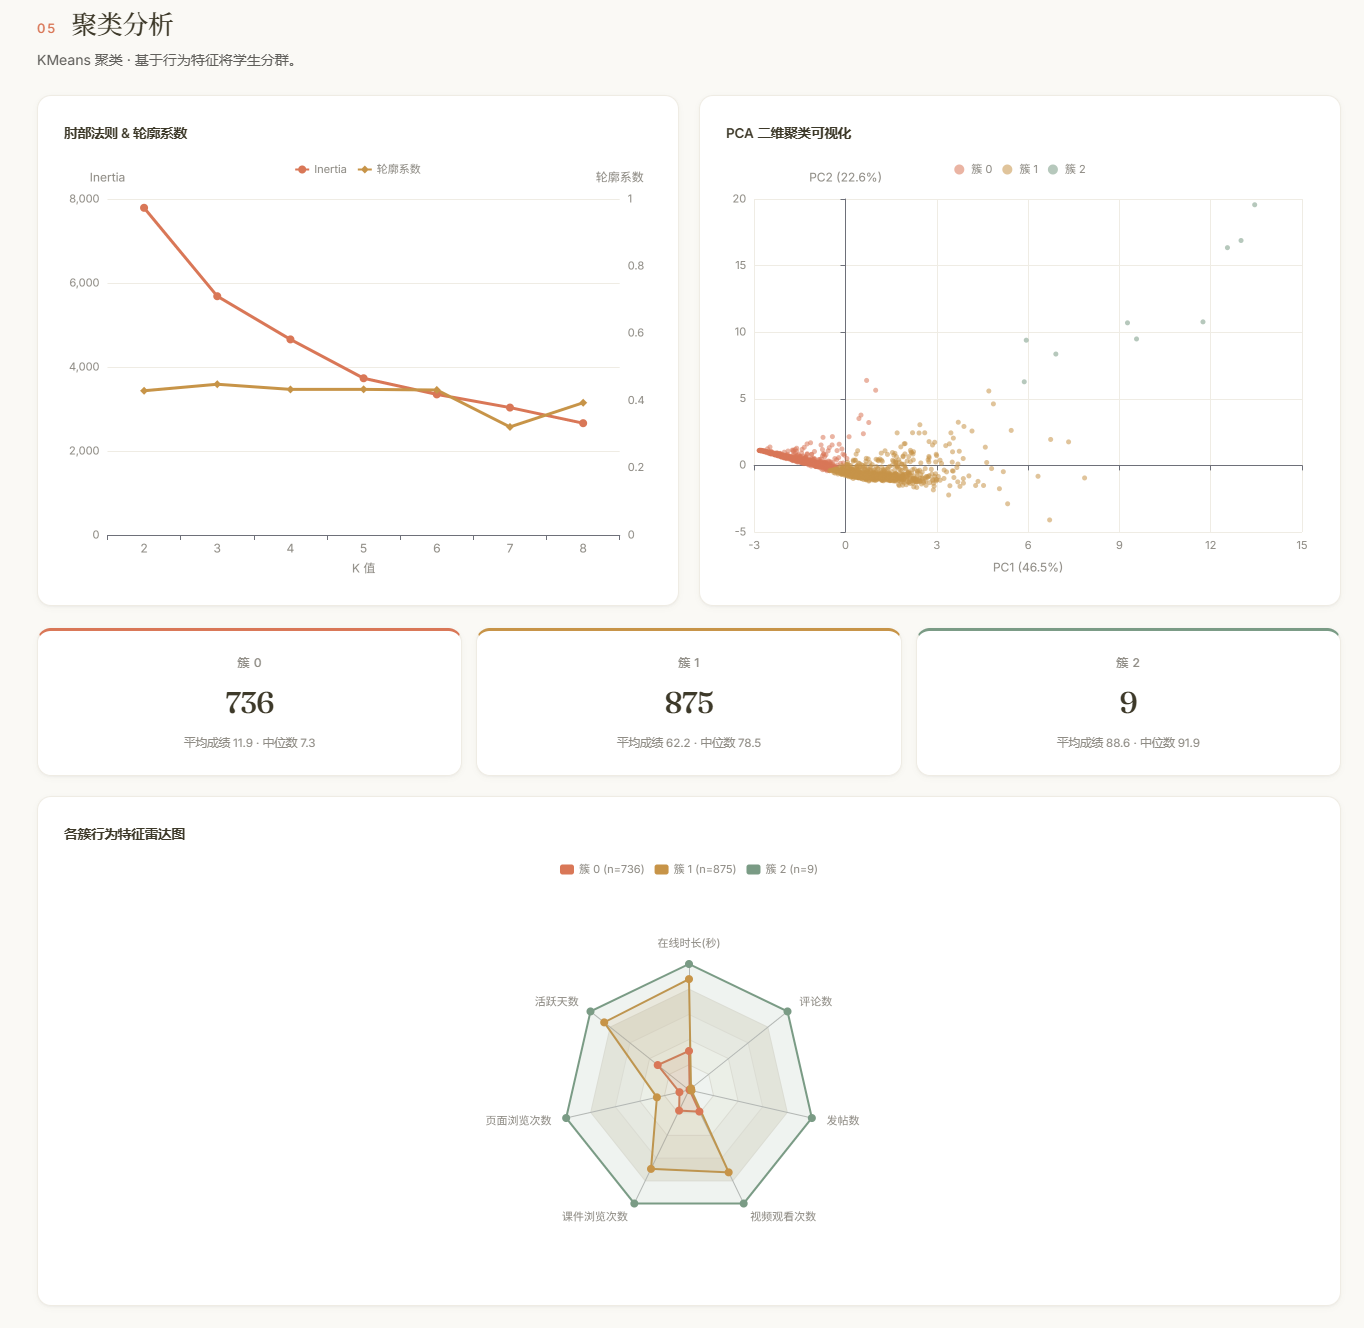
\includegraphics[width=\textwidth]{Kmeans.png}
    \caption{聚类分析页面}
    \label{fig:webview_kmeans}
\end{subfigure}\hfill
\begin{subfigure}{0.48\textwidth}
    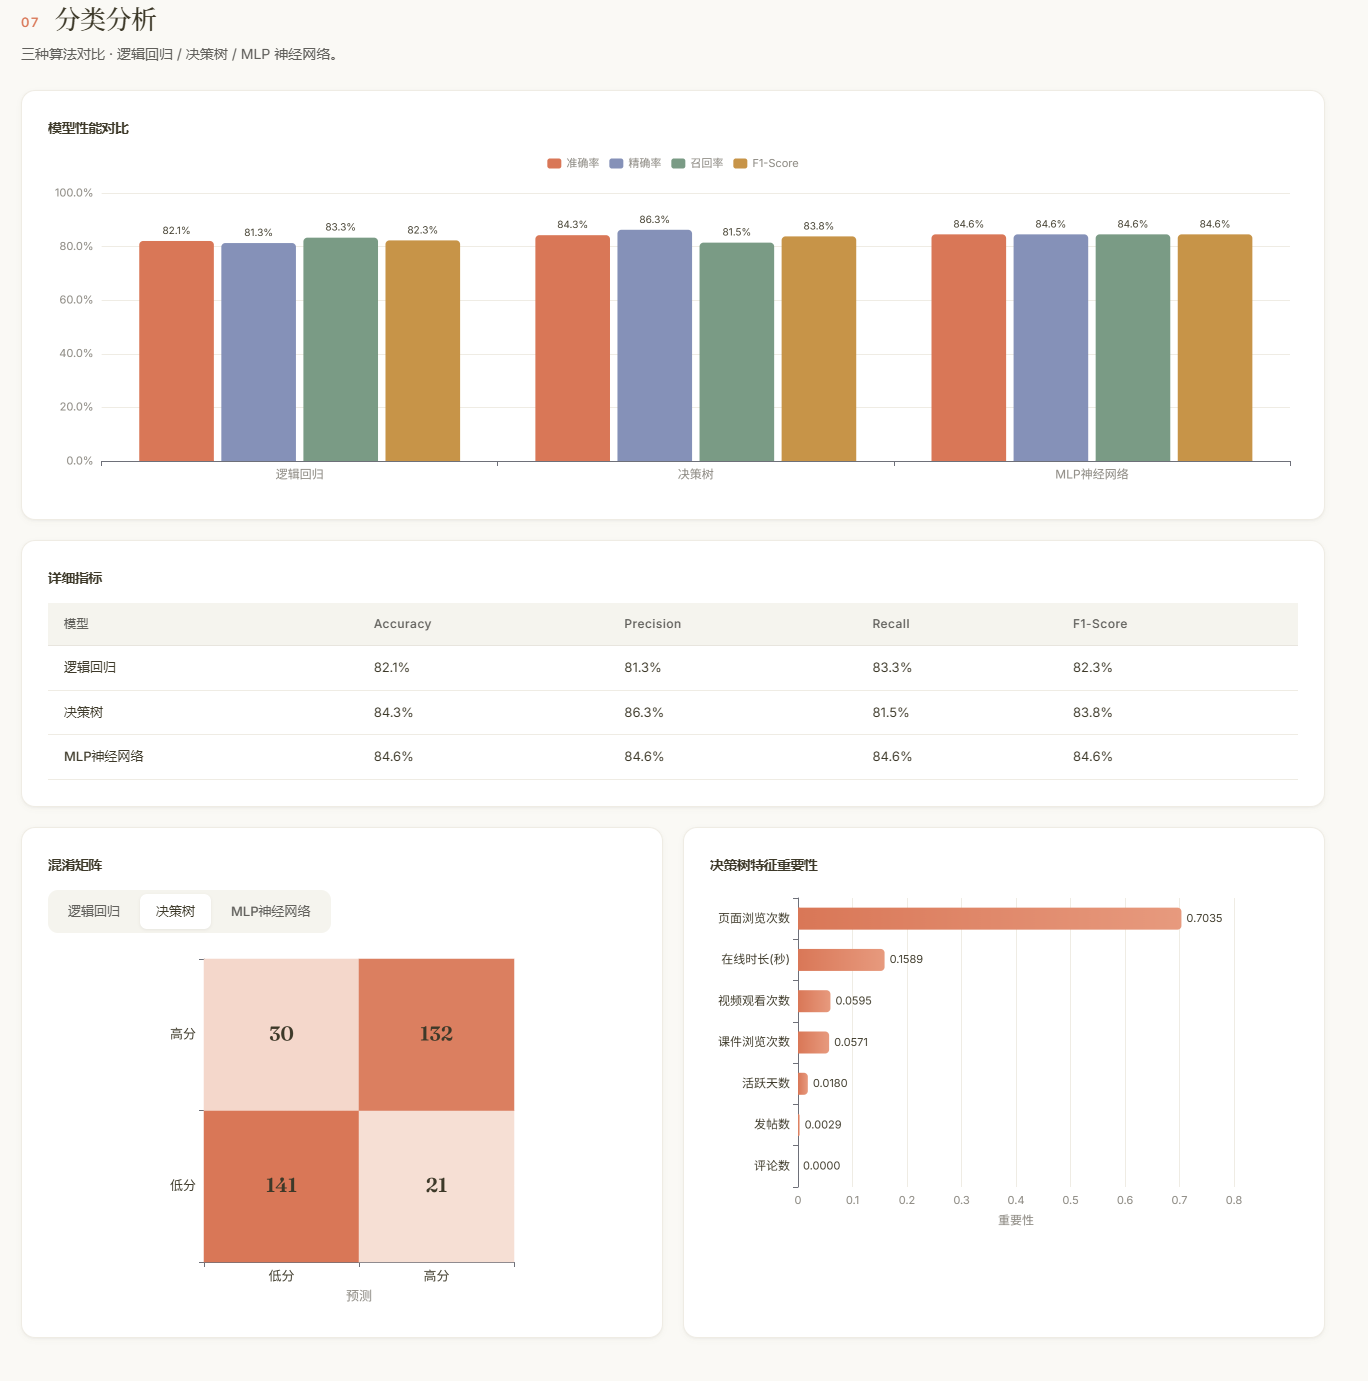
\includegraphics[width=\textwidth]{compares.png}
    \caption{分类模型对比页面}
    \label{fig:webview_cls}
\end{subfigure}
\caption{EduAnalytics 聚类与分类分析页面}
\label{fig:webview_analysis2}
\end{figure}

\begin{figure}[H]
\centering
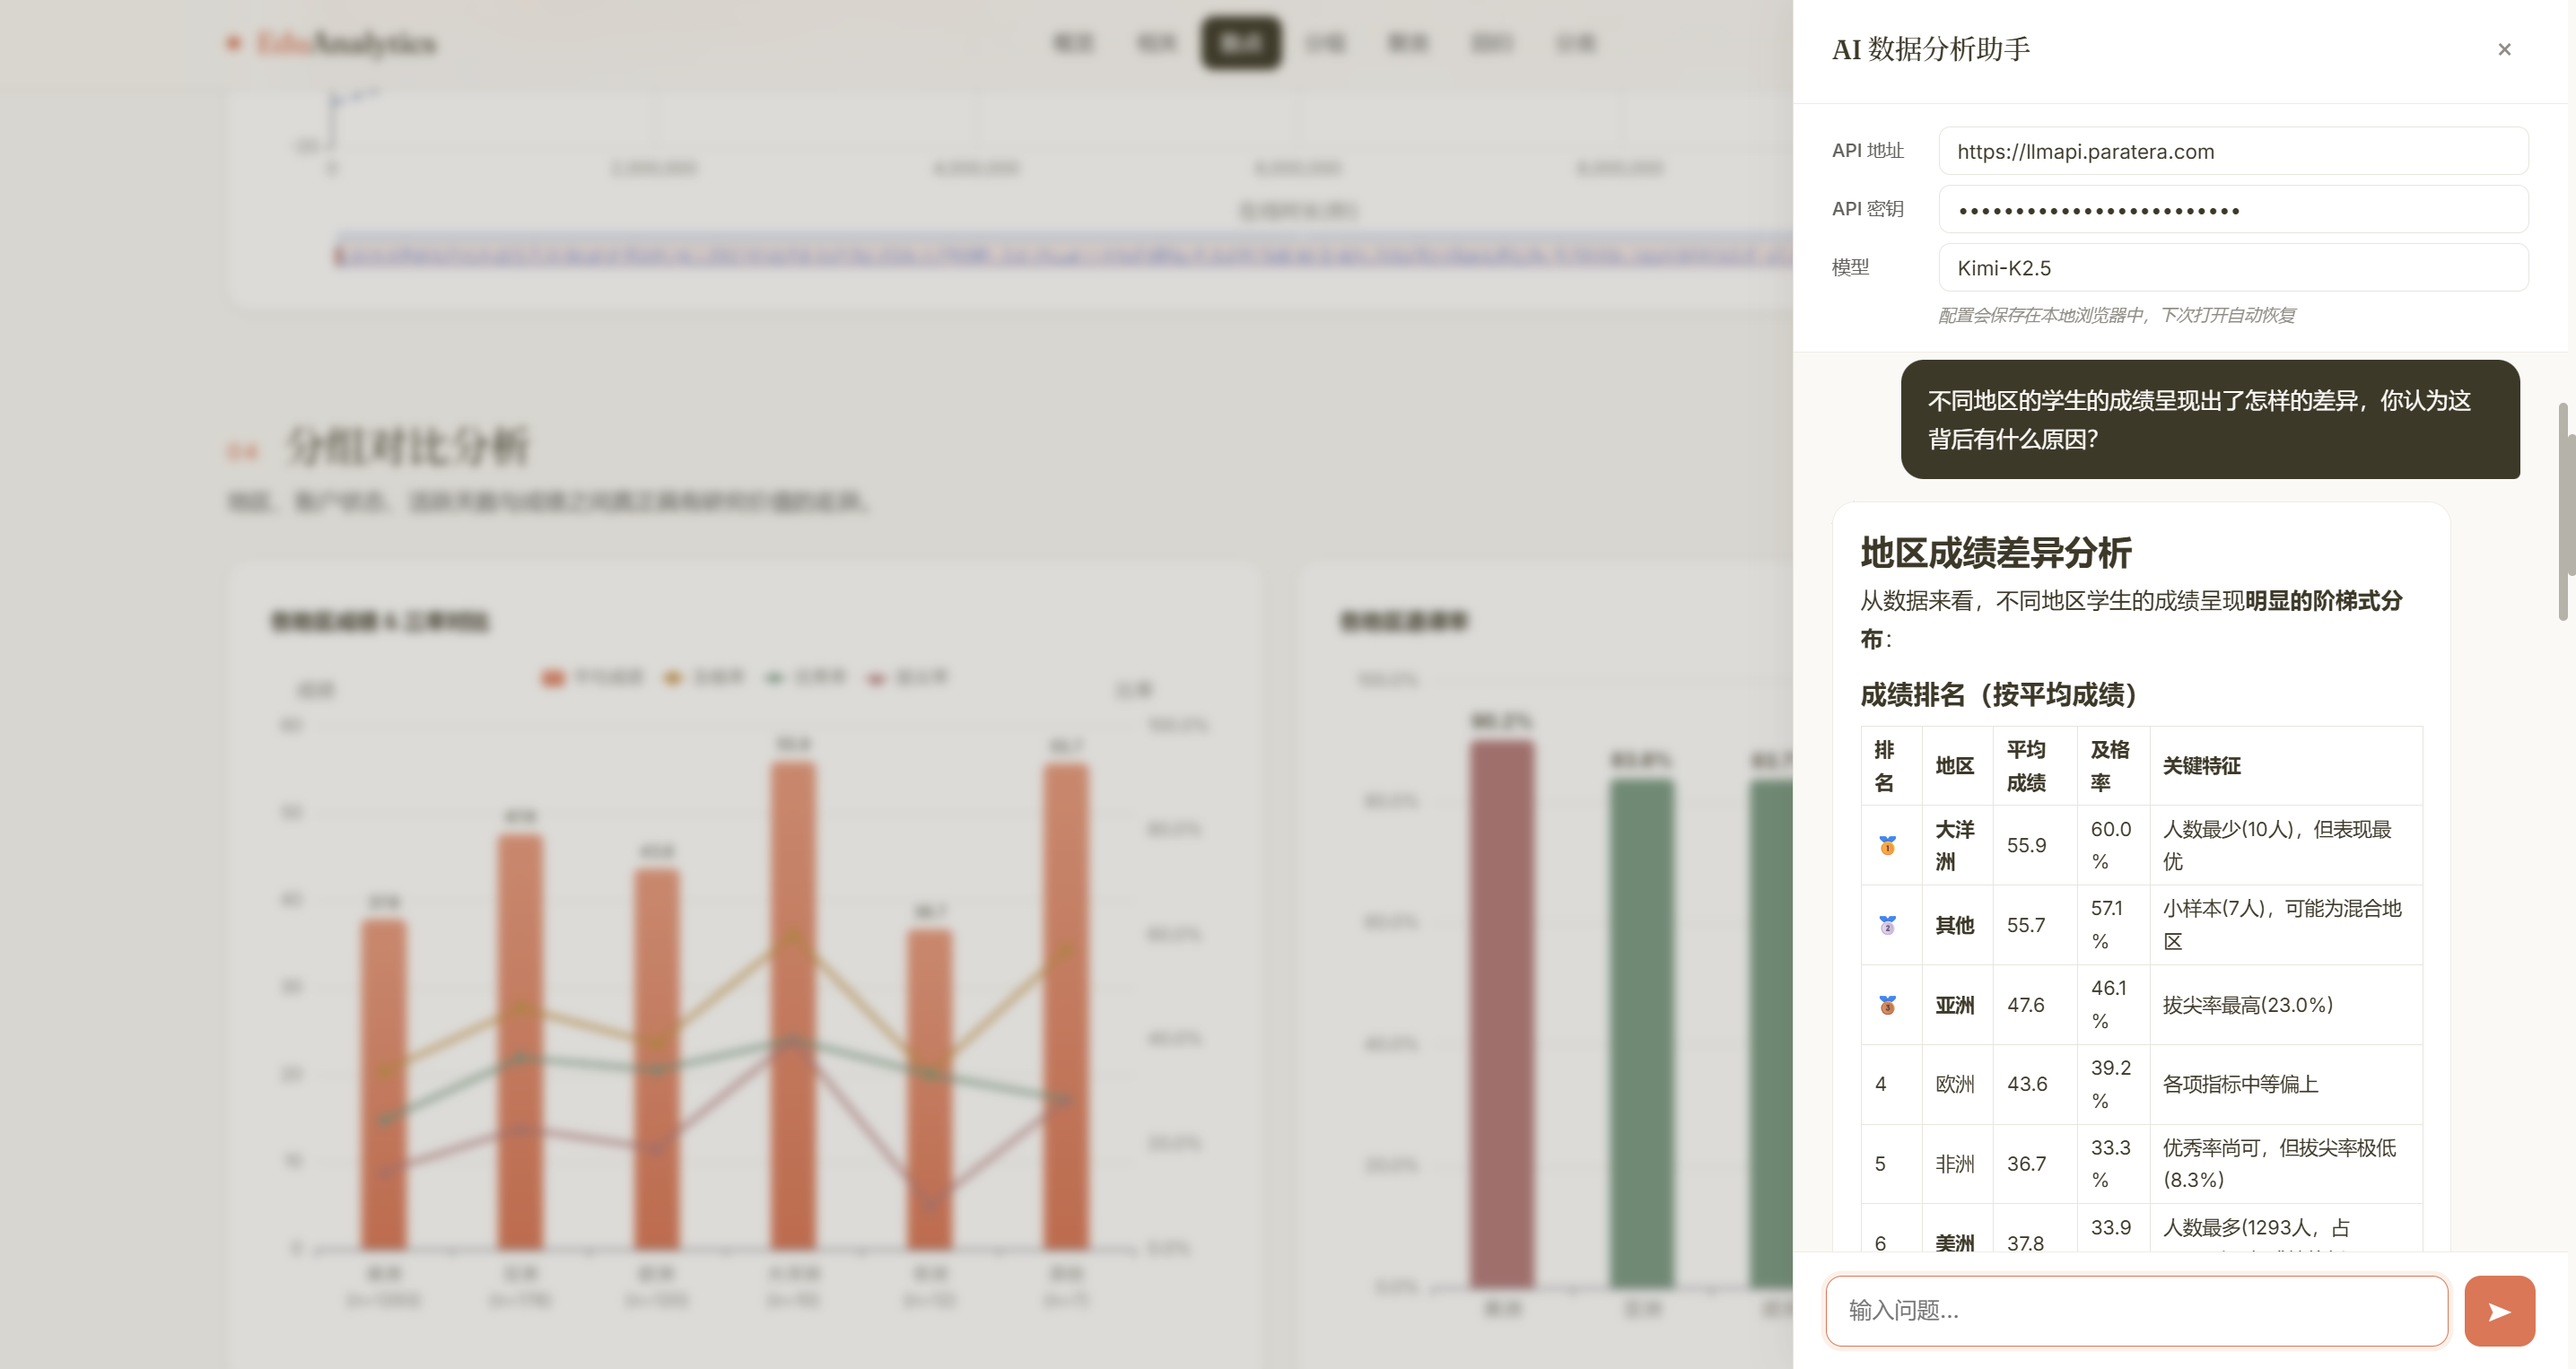
\includegraphics[width=0.96\textwidth]{ai_1.png}
\caption{AI 助手对话界面：侧边栏布局、API 配置区与对话主体}
\label{fig:ai_chat_1}
\end{figure}

\begin{figure}[H]
\centering
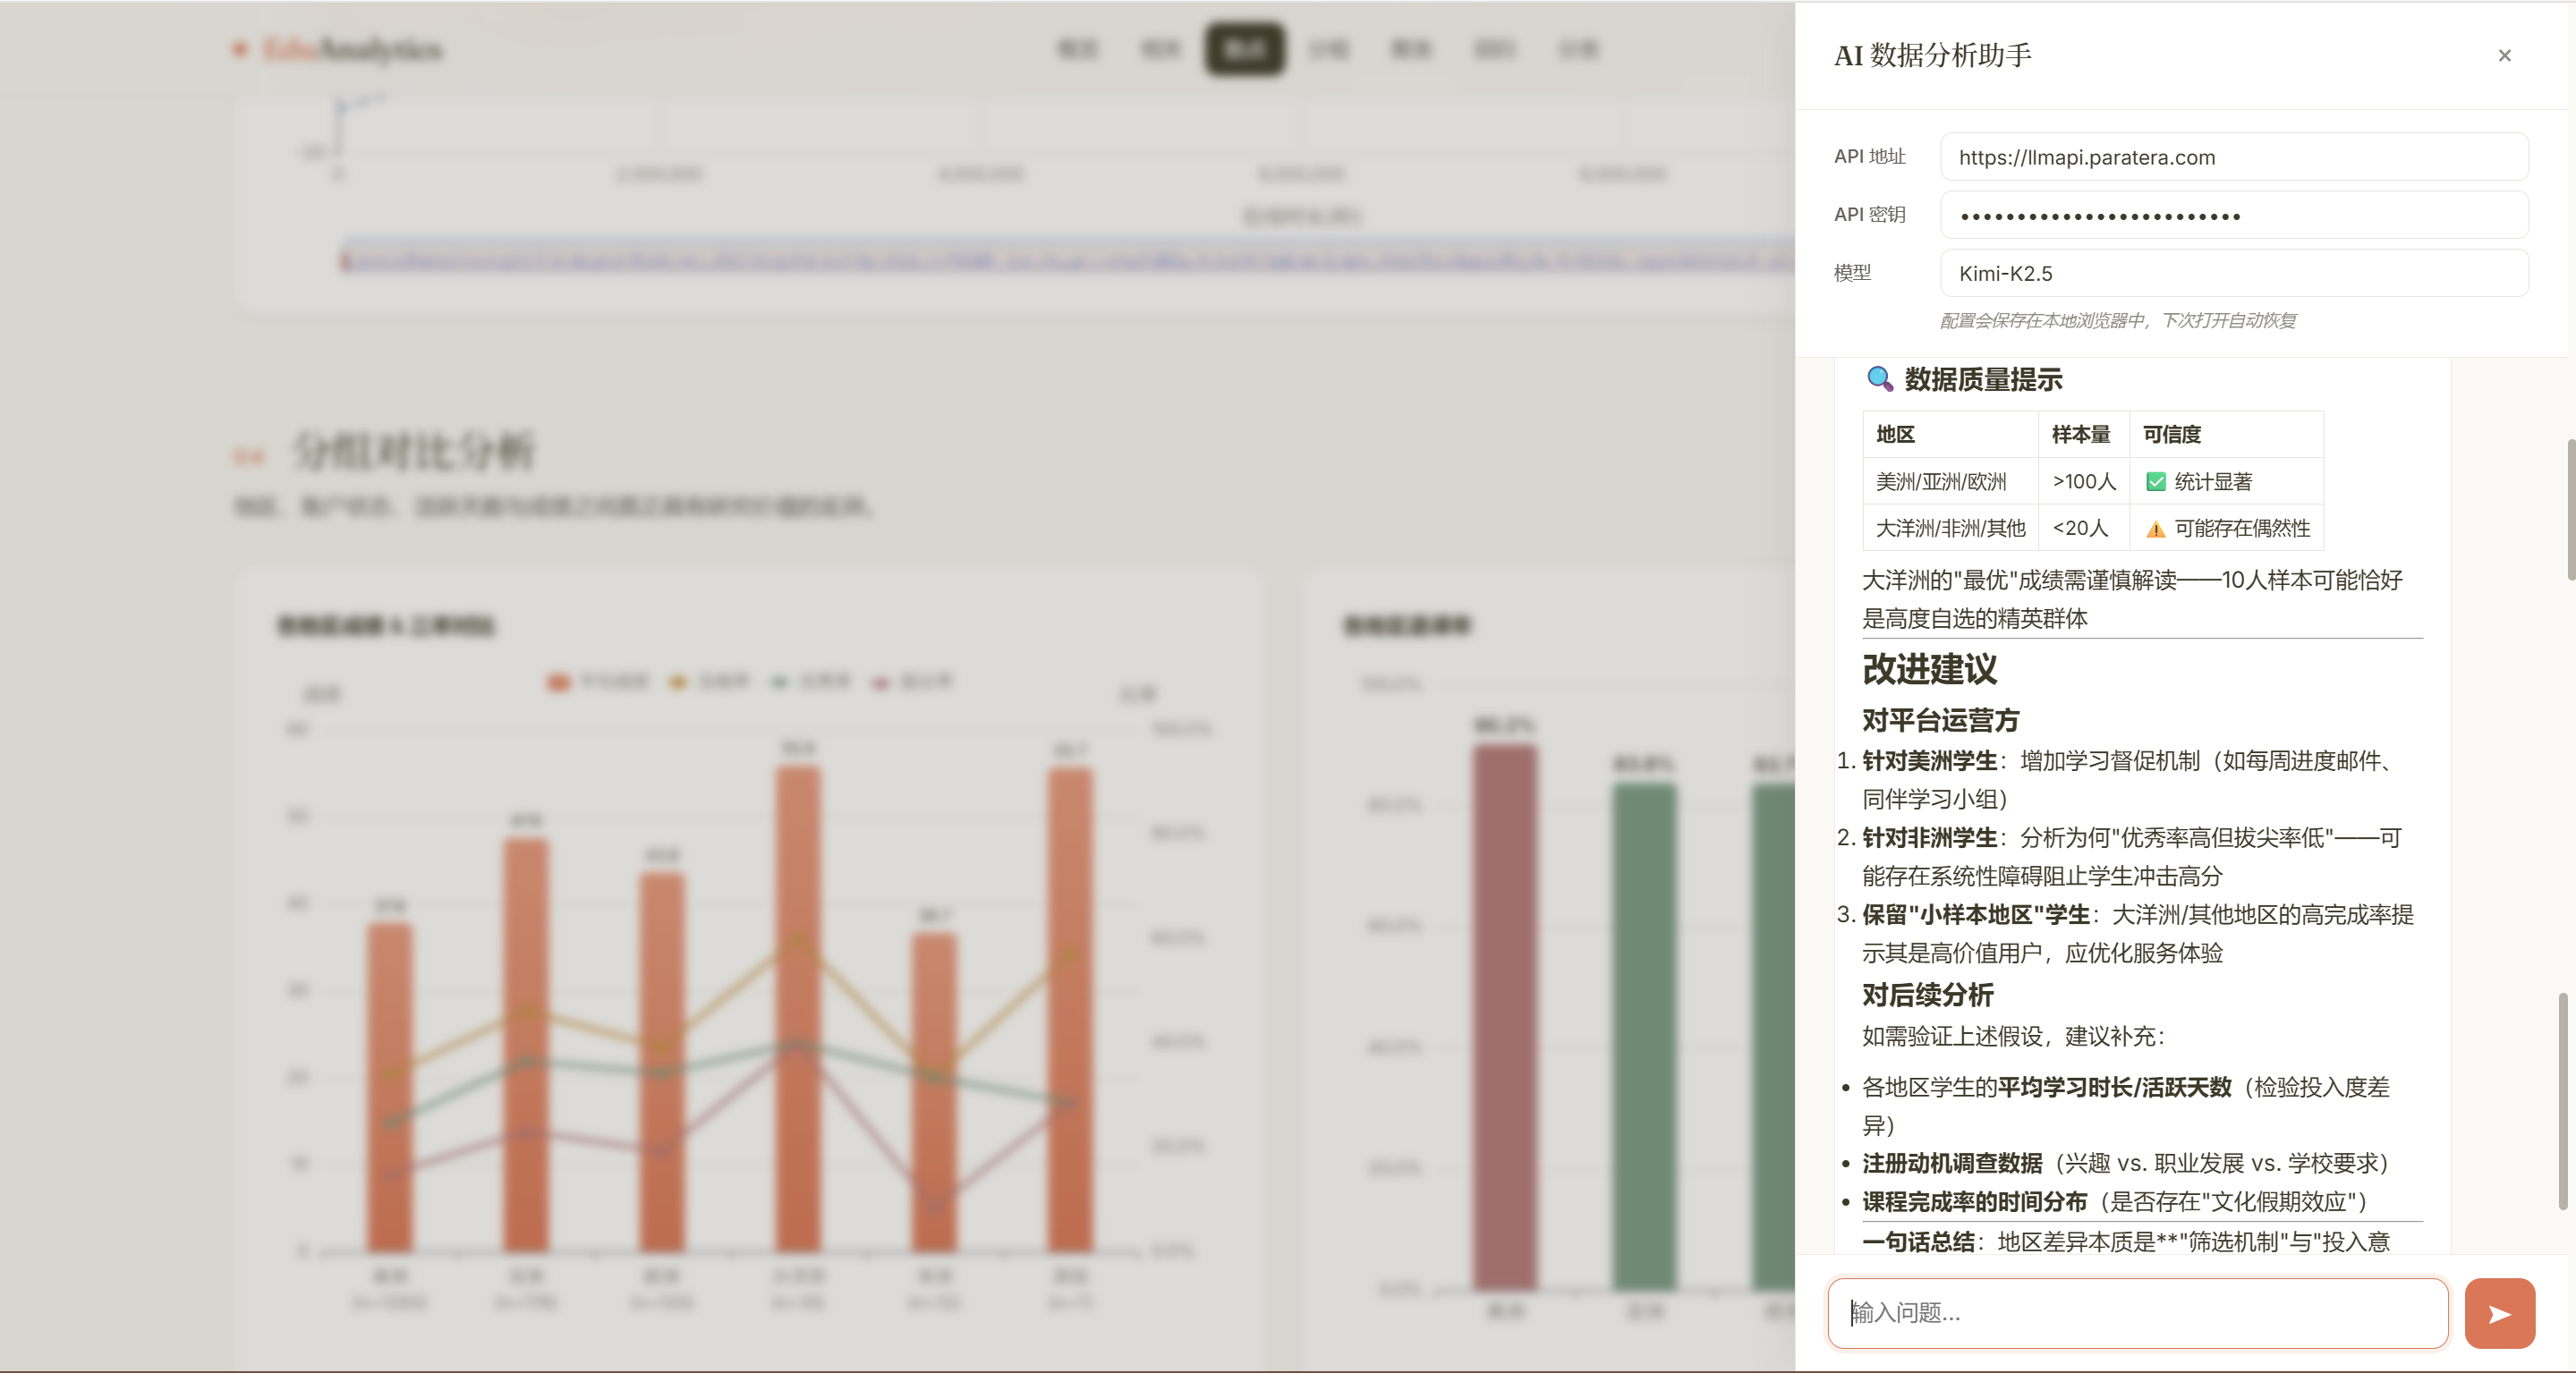
\includegraphics[width=0.96\textwidth]{ai_2.png}
\caption{AI 助手基于当前数据集的结构化回答示例（支持 Markdown 表格与代码块）}
\label{fig:ai_chat_2}
\end{figure}

\subsection{使用方法}

最便捷的方式是直接访问已部署的在线版本 \url{https://eduanalytics-qpq7.onrender.com/}，跳过环境配置直接进入使用流程的第三步。若希望在本地运行（例如用于离线场景或二次开发），完整流程如下：
\begin{enumerate}
    \item \textbf{环境准备（首次本地使用）}：克隆仓库后在项目根目录执行\\
          \indent\indent\texttt{uv sync}\\
          即可自动创建虚拟环境并安装锁定版本的依赖；若未安装\texttt{uv}，亦可依次执行\\
          \indent\indent\texttt{python -m venv .venv}\\
          \indent\indent\texttt{source .venv/bin/activate}\\
          \indent\indent\texttt{pip install -r requirements.txt}\\
          作为替代方案。
    \item \textbf{启动服务}：在项目根目录下执行\\
          \indent\indent\texttt{uv run python app.py}\\
          （或激活虚拟环境后运行 \texttt{python app.py}），随后在浏览器打开 \url{http://localhost:5000}。
    \item \textbf{上传数据}：将包含 \texttt{grade} 列的CSV文件拖入页面中央的虚线框，或点击按钮选择文件；数据大小上限为64\,MB。上传成功后页面自动刷新进入分析视图。
    \item \textbf{浏览分析}：通过顶部导航栏或页面滚动在七个分析章节间跳转，所有图表均支持悬停查看细节、框选数据区域以及缩放等交互。
    \item \textbf{AI 问答（可选）}：点击右上角“AI 助手”按钮展开侧边栏。首次使用时填写API地址（如\url{https://api.openai.com/v1}）、API密钥与模型名；之后直接输入问题，助手会基于当前数据集回答关于学习行为、特征关系、群体差异等问题。若需更换数据集，可在英雄区点击“更换文件”按钮清空当前状态并重新上传。
\end{enumerate}

\subsection{与离线脚本的差异}

相较于本课题最初版本的 \texttt{data\_analyse.py} 离线脚本——输出一组静态的CSV、TXT和PNG文件——EduAnalytics 在工作流、交互性和复用性上均有明显提升，对比如表\ref{tab:cli_vs_web}所示。
\begin{table}[H]
\centering
\caption{离线脚本与在线平台的对比}
\label{tab:cli_vs_web}
\begin{tabular}{lll}
\toprule
\textbf{维度} & \textbf{data\_analyse.py} & \textbf{EduAnalytics} \\
\midrule
数据来源   & 硬编码CSV路径     & 浏览器拖拽上传 \\
输出形式   & 多个静态文件      & 单页交互式仪表盘 \\
图表交互   & 静态PNG          & 悬停/缩放/筛选 \\
AI能力     & 无               & LLM 问答（数据感知） \\
复用性     & 绑定单一数据集   & 任意CSV即开即用 \\
\bottomrule
\end{tabular}
\end{table}

% ══════════════════════════════════════════════════════════════════════════
\section{结论与展望}
% ══════════════════════════════════════════════════════════════════════════

\subsection{主要结论}

本研究基于Coursera MOOC平台的15,168条学生数据，系统分析了在线学习行为与成绩之间的关系。主要结论如下：

\begin{enumerate}
    \item \textbf{高退课率是MOOC面临的首要挑战}。数据集中89.3\%的学生成绩为0（退课），仅1,620人实际参与学习。
    \item \textbf{在线时长、活跃天数和页面浏览是影响成绩的最关键行为特征}，与成绩的Pearson相关系数均超过0.67。论坛参与的影响相对较弱。
    \item \textbf{K-Means聚类将学生有效划分为三个群体}：低活跃-低成绩组（45.4\%）、中高活跃-中高成绩组（54.0\%）和极高活跃-高成绩组（0.6\%），轮廓系数为0.449。
    \item \textbf{行为特征能够较好地预测成绩}。线性回归模型$R^2=0.614$；MLP分类模型准确率达84.57\%。
    \item \textbf{配套平台将本研究方法论具象化为可交互工具}。EduAnalytics 将离线脚本升级为可在浏览器中拖拽使用的Web应用，并引入数据感知的AI问答，使分析结果易于被非编程用户复用。
\end{enumerate}

\subsection{实践建议}

基于分析结果，对在线教育平台提出以下建议：
\begin{itemize}
    \item 建立基于在线时长和活跃天数的\textbf{早期预警系统}，及时识别可能退课或成绩不佳的学生。
    \item 通过游戏化设计、定期提醒等方式\textbf{鼓励持续学习}，提高学生的活跃天数。
    \item 优化论坛设计以\textbf{提升互动参与度}，使其对成绩产生更大的正向影响。
\end{itemize}

\subsection{研究局限与展望}

本研究存在以下局限：（1）数据来源于单一课程，结论的泛化性需要进一步验证；（2）仅使用了线性和浅层模型，更复杂的模型（如梯度提升树、深度学习）可能取得更好的预测效果；（3）未考虑时间序列特征，如学习节奏的变化趋势。

未来研究方向包括：引入时序分析方法捕捉学习行为的动态变化，结合自然语言处理分析论坛文本内容，以及在多课程、多平台数据上验证模型的泛化能力。

% ══════════════════════════════════════════════════════════════════════════
\section*{致谢}
% ══════════════════════════════════════════════════════════════════════════

感谢北京大学 2026 年春季《教育与人工智能》课程团队提供的数据集与课程指导，感谢课程主讲教师贾积有教授在研究选题、分析方法与平台设计上的悉心指导，也感谢课程助教在作业过程中给予的答疑与帮助。

% ══════════════════════════════════════════════════════════════════════════
\renewcommand{\refname}{参考文献}
\bibliographystyle{unsrt}
\bibliography{references}
% ══════════════════════════════════════════════════════════════════════════

\end{document}
